%%%%%%%%%%%%%%%%%%%%%%%%%%%%%%%%%%%%%%%%%%%%%%%%%%%%%%%%%%%%%%%%%%%%%%%
% Created on Mon June 5, 2023
% @author: Giselle Labrador Badia (@gisslab)
%
% This report analyses OB auction files for the early Covid period. 
% It is based on the code files auction_prices_analysis.py, 
% auction_prices_timeseries_plots, fed_mbs
%%%%%%%%%%%%%%%%%%%%%%%%%%%%%%%%%%%%%%%%%%%%%%%%%%%%%%%%%%%%%%%%%%%%%%%




\documentclass[11pt,a4paper]{article}


\usepackage[utf8]{inputenc}
\usepackage[spanish,english]{babel}
\usepackage{apacite}
\usepackage[round]{natbib}
\usepackage{hyperref}
\bibliographystyle{apacite}


\usepackage[margin = 1in, top=1.5cm,bottom=1.5cm]{geometry}% Margins
\setlength{\parindent}{2em}
\setlength{\parskip}{0.3em}
\usepackage{setspace} % Setting the spacing between lines
\usepackage{hyperref} % To create hyperlinks within the document
\spacing{1.15}

%images
\usepackage{graphicx}
% \usepackage{subcaption}
\usepackage{caption}
% subcaption was interfering with the figure count, fix below
\usepackage{subcaption, xparse}

% to read mid rule
\usepackage{booktabs}

\usepackage[capposition=top]{floatrow}
\captionsetup[sub]{font=footnotesize,labelfont={bf,sf}}

\begin{document}

\title{Analysis of Auctions in OB in the Early Covid Period}

\maketitle



\section{FED purchases of MBS}

The following figures show the daily time series of amounts and prices of FED purchases of MBAs for FNMA products and 30-year maturity in the early COVID period.

\begin{figure}[h]
    \centering
    \begin{subfigure}[b]{0.49\textwidth}
      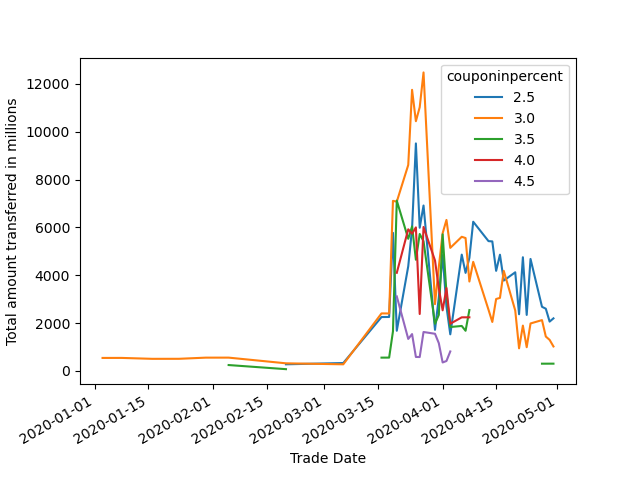
\includegraphics[width=0.998\textwidth]{../results/figures/FNMA_daily_purchases_tradedate_amount.png}
      \caption{ Quantity by trade date}
     \end{subfigure}
     \begin{subfigure}[b]{0.49\textwidth}
      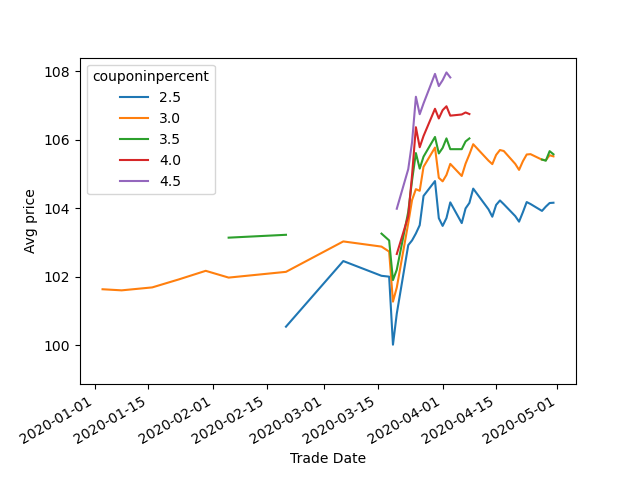
\includegraphics[width=0.998\textwidth]{../results/figures/FNMA_daily_purchases_tradedate_price.png}
      \caption{ Price by trade date}
     \end{subfigure}
    \begin{subfigure}[b]{0.49\textwidth}
        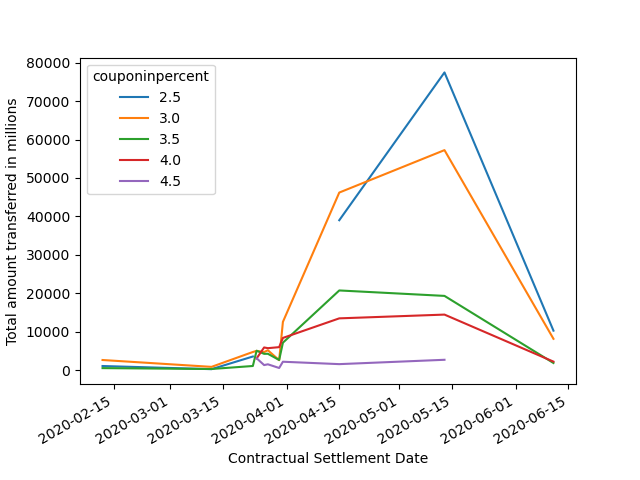
\includegraphics[width=0.998\textwidth]{../results/figures/FNMA_daily_purchases_contractualsettlementdate_amount.png}
        \caption{ Quantity by settlement date}
       \end{subfigure}
       \begin{subfigure}[b]{0.49\textwidth}
        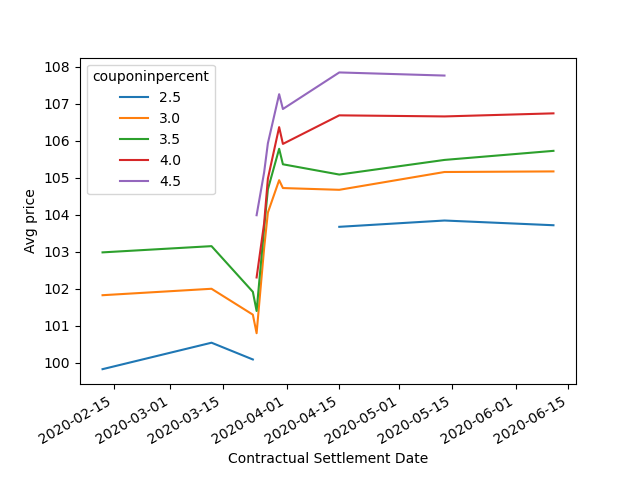
\includegraphics[width=0.998\textwidth]{../results/figures/FNMA_daily_purchases_contractualsettlementdate_price.png}
        \caption{ Price by settlement date}
       \end{subfigure}
     \caption{FED purchases of FNMA products in the early COVID period} 
     \begin{minipage}{\textwidth}
        \footnotesize{\textit{Notes:} The figure shows the daily time series of amounts and prices of FED purchases of FNMA products and 30-year maturity. Colors represent different coupons. } 
        \end{minipage}
\end{figure}

\pagebreak
\section{OB Auctions in the Early Covid Period}

The following figure shows a histogram of all bids for all auctions in the OB platform between January 2020 and December 2021. 
The product is Conforming loans with a 30-year maturity. 


%figure 

\begin{figure}[h]
    \centering
    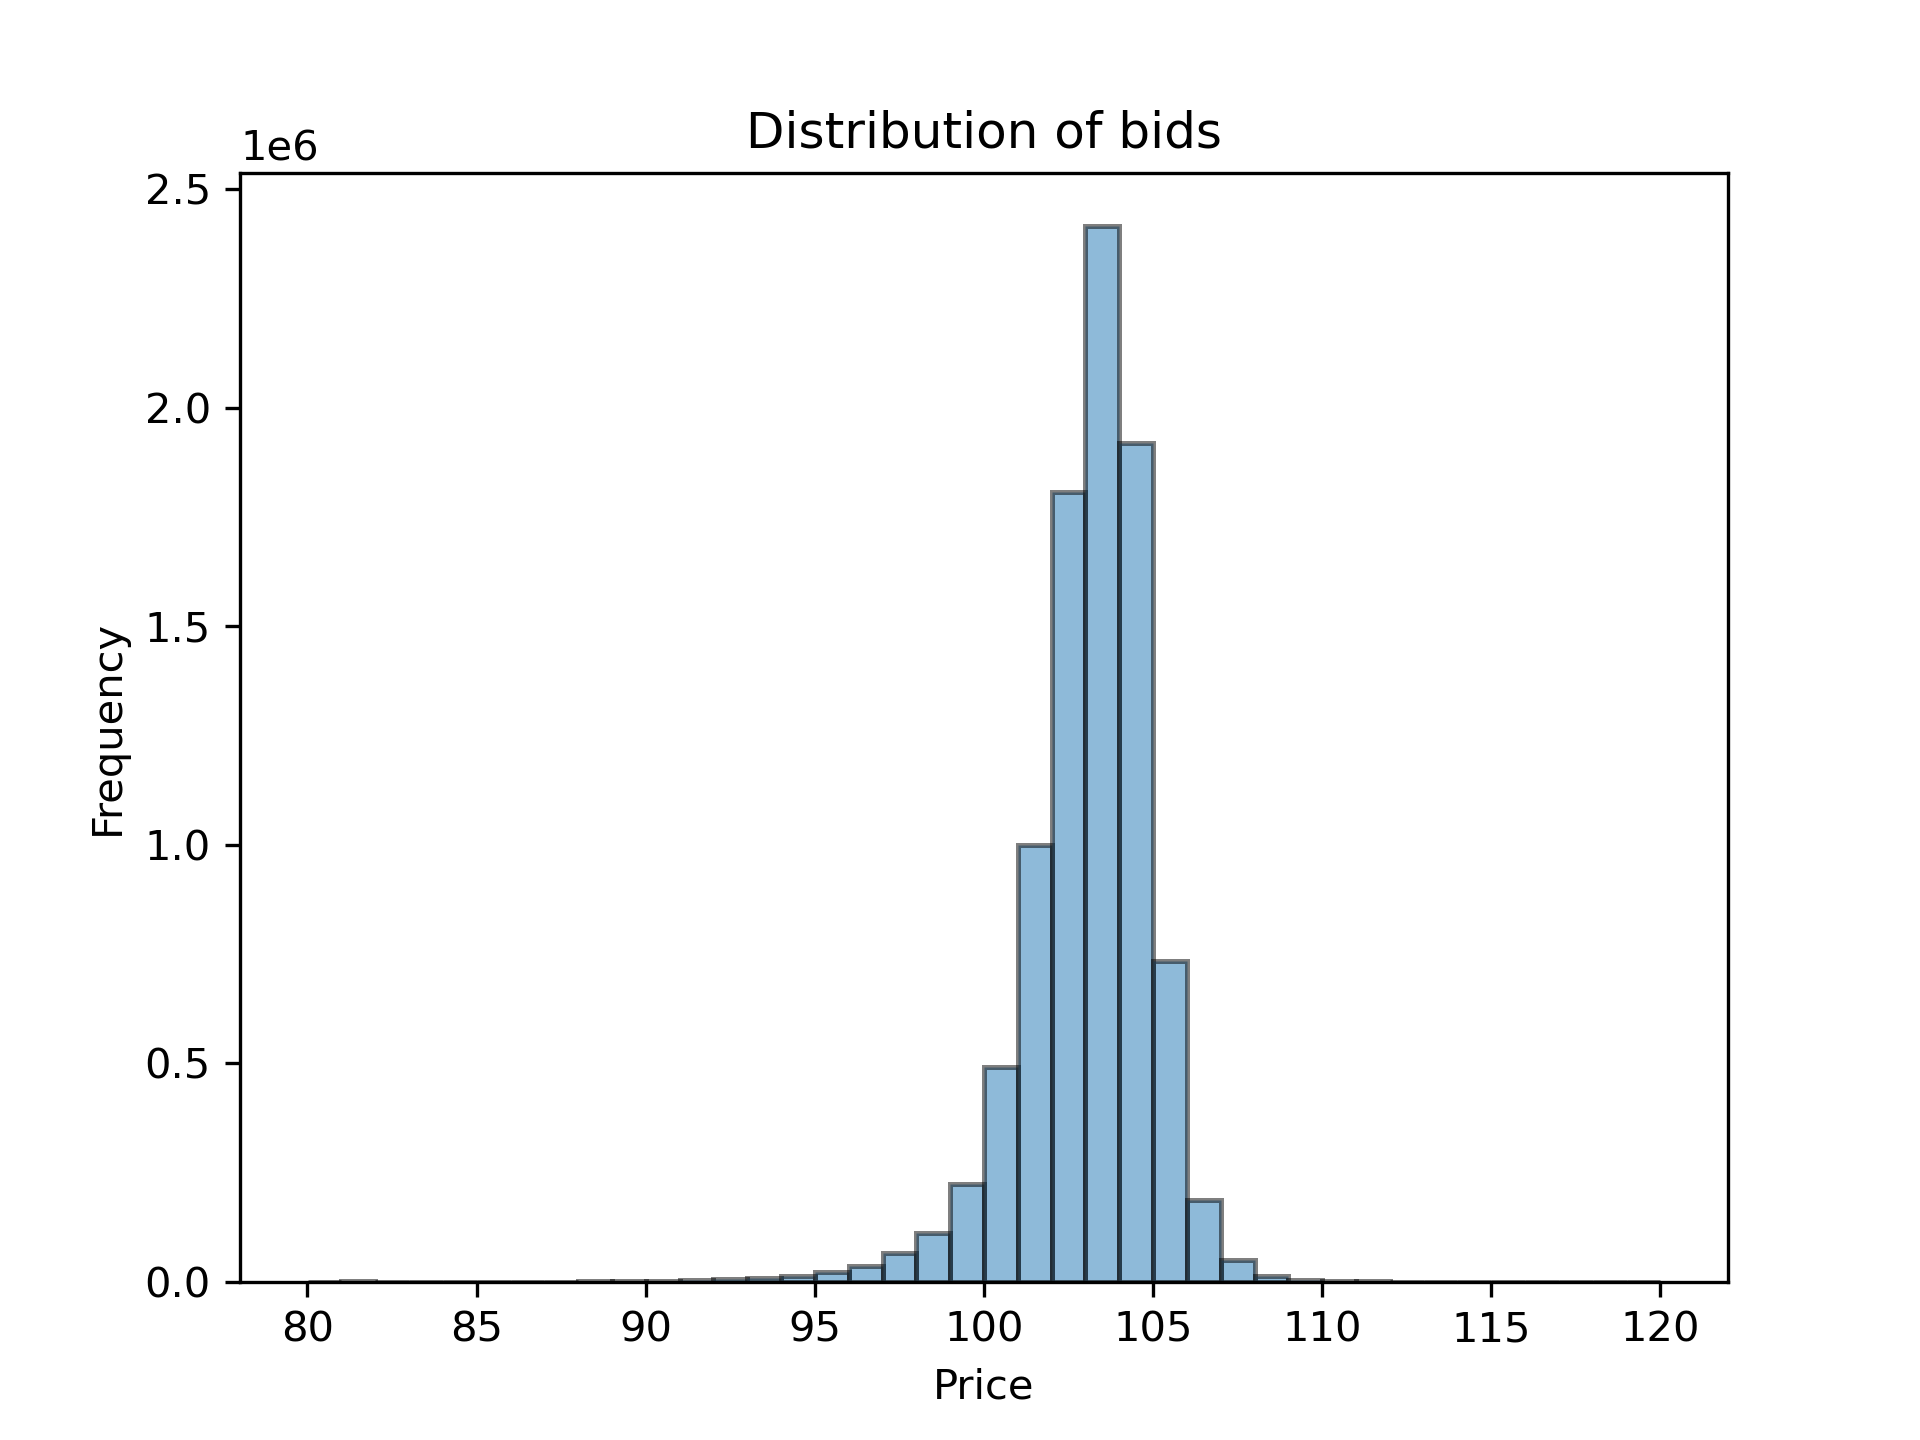
\includegraphics[width=0.62\textwidth]{../results/figures/distribution_of_bids.png}
    \caption{Histogram of all bids for all auctions in the oB platform for the months of January, February, March, and April 2020. The product is Conforming loans with a 30-year maturity.}
    \begin{minipage}{\textwidth}
        \footnotesize{\textit{Notes:} The figure shows a histogram of all bids for all auctions in the OB platform for the months of January, February, March, and April 2020. The product is Conforming loans with a 30-year maturity. } 
        \end{minipage}
\end{figure}

This figure shows a histogram for the note rates by auction for the same period and product.
\begin{figure}[h]
  \centering
  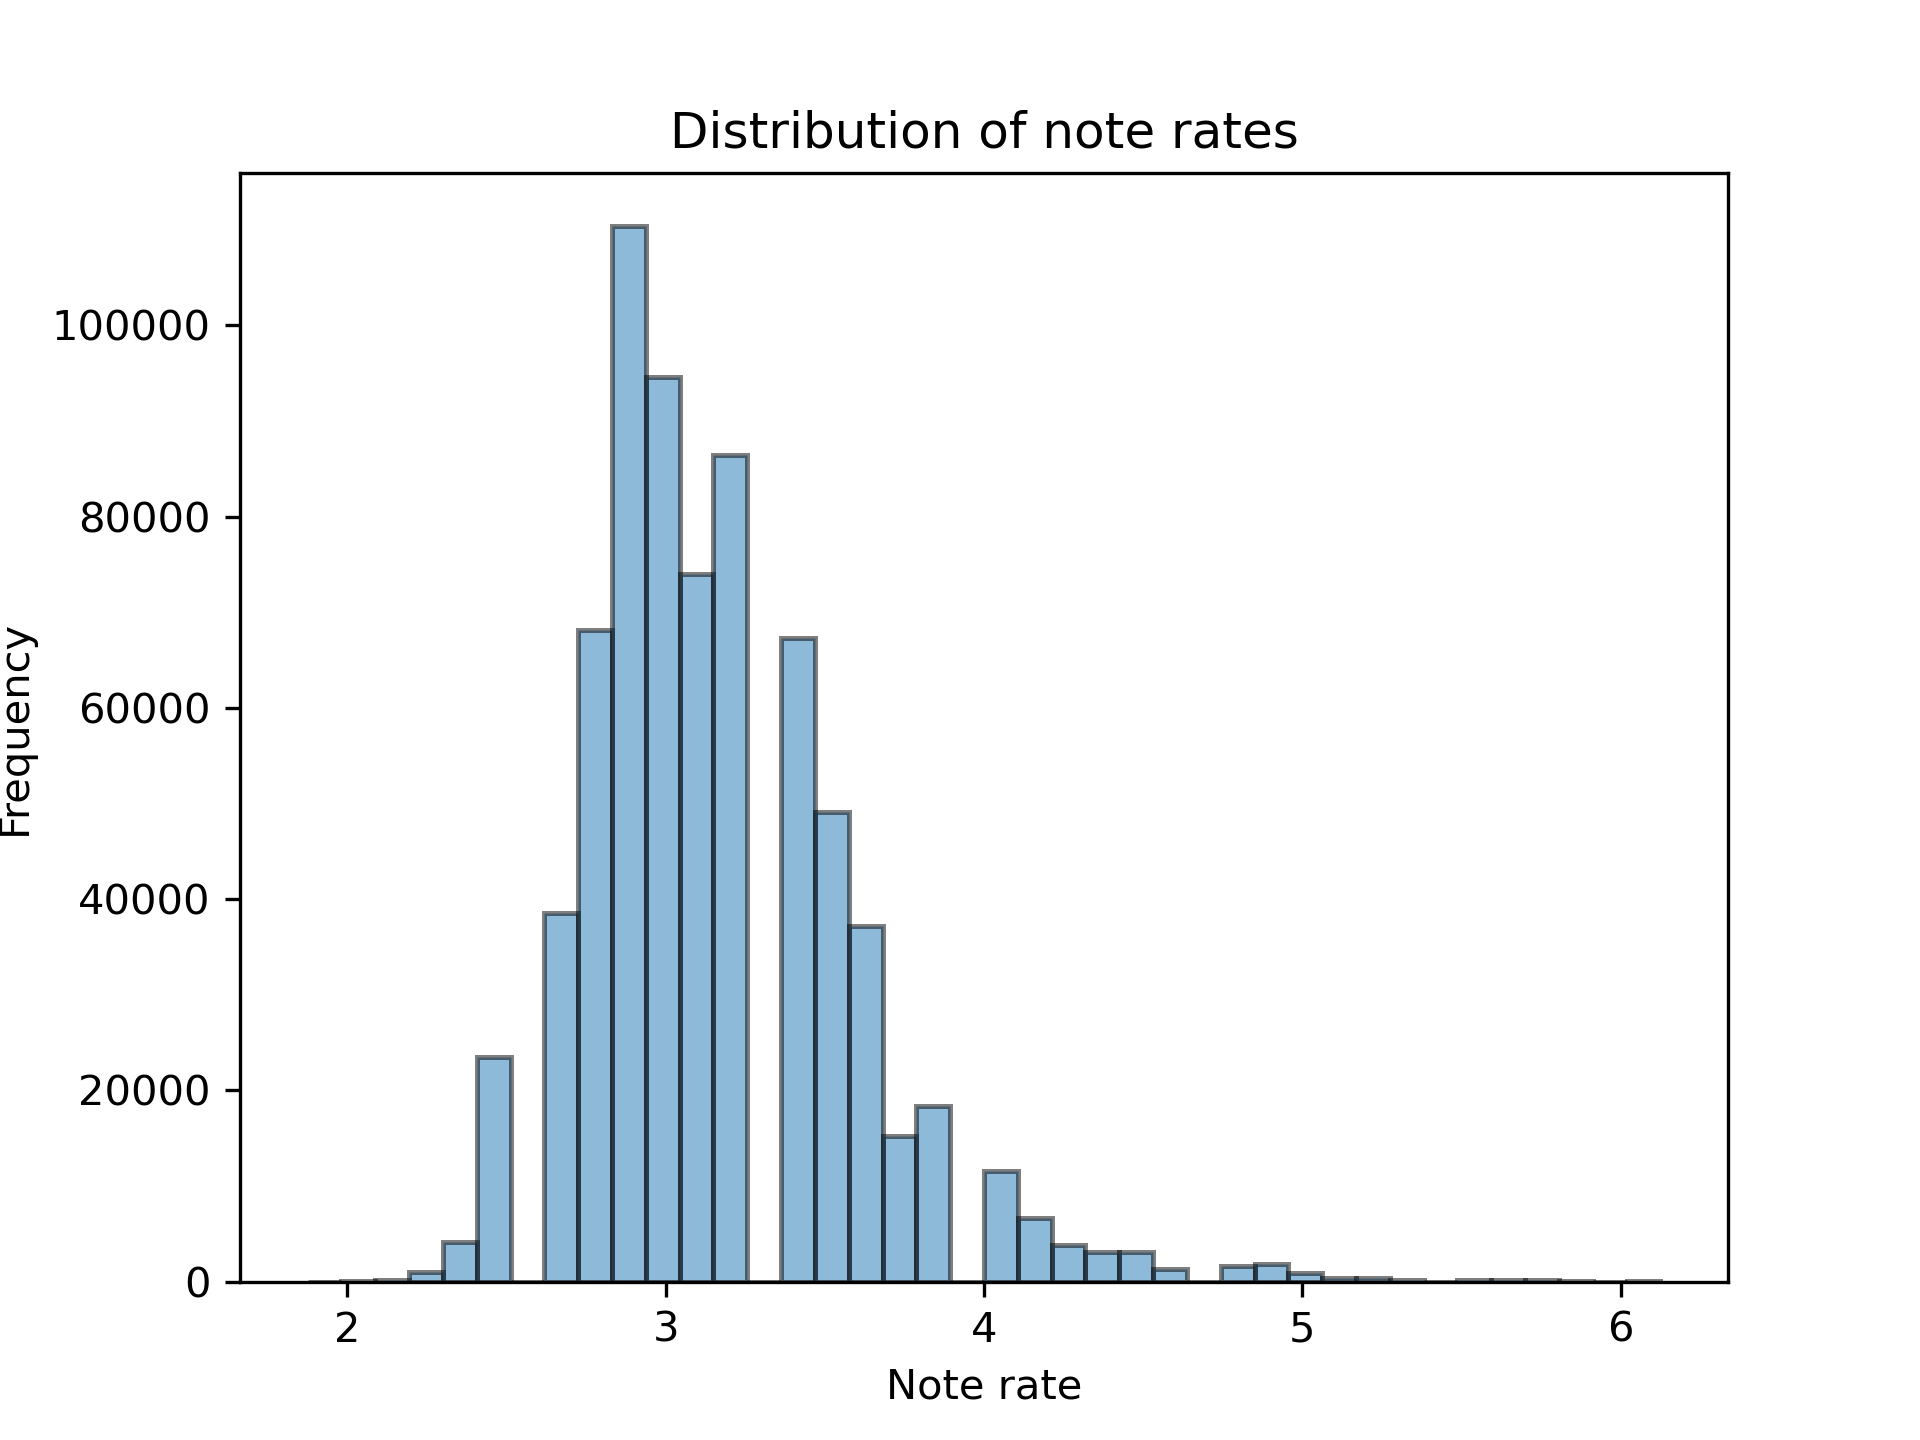
\includegraphics[width=0.62\textwidth]{../results/figures/distribution_of_noterates.png}
  \caption{Histogram of all bids for all auctions in the oB platform for the months of January, February, March, and April 2020. The product is Conforming loans with a 30-year maturity.}
  \begin{minipage}{\textwidth}
      \footnotesize{\textit{Notes:} The figure shows a histogram of all note rates of auctioned loans in the OB platform for the months of January, February, March, and April 2020. The product is Conforming loans with a 30-year maturity. } 
      \end{minipage}
\end{figure}


\pagebreak
Table 1 shows descriptive statistics for important outcomes at the auction level for the same period and product. 

%table

\begin{table}[h]
    \centering
    \begin{tabular}{lrrrrrrrr}
\toprule
{} &    count &    mean &     std &     min &     25\% &  median &     75\% &      max \\
\midrule
Loan amount            &  80848.0 &  274.37 &  126.61 &   23.25 &  179.74 &  257.00 &  354.33 &  1470.00 \\
Note rate              &  80848.0 &    3.71 &    0.45 &    2.25 &    3.38 &    3.62 &    3.88 &     6.12 \\
Price                  &  80848.0 &  104.04 &    1.36 &   94.03 &  103.25 &  104.02 &  104.82 &   120.00 \\
Days to auction        &  80704.0 &    4.76 &    7.96 & -326.00 &    1.00 &    3.00 &    6.00 &   288.00 \\
Number of participants &  80848.0 &   11.35 &    5.52 &    1.00 &    8.00 &   12.00 &   15.00 &    32.00 \\
Number of bulk bidders &  80848.0 &    7.37 &    6.08 &    0.00 &    0.00 &    8.00 &   12.00 &    27.00 \\
Sell rate              &  80848.0 &    0.77 &    0.42 &    0.00 &    1.00 &    1.00 &    1.00 &     1.00 \\
Rate sell to winner    &  80848.0 &    0.49 &    0.50 &    0.00 &    0.00 &    0.00 &    1.00 &     1.00 \\
\bottomrule
\end{tabular}

    \caption{Descriptive statistics at the auction level. }
    \begin{minipage}{\textwidth}
        \footnotesize{\textit{Notes:} The table shows descriptive statistics at the auction level of observation for the months of January, February, March, and April 2020. The product is Conforming loans with a 30-year maturity. } 
        \end{minipage}
\end{table}

% \pagebreak

\subsection{Naive comparison before after COVID}

A similar table is depicted for the months of January and February and for the months of March and April. The idea is to compare the outcomes before and after COVID (tables 2 and 3 respectively).

%table
\begin{table}[h]
  \centering
  \begin{tabular}{lrrrrr}
\toprule
{} &    count &    mean &     std &     min &      max \\
\midrule
Loan amount            &  28572.0 &  261.97 &  126.40 &   23.25 &  1184.92 \\
Note rate              &  28572.0 &    3.98 &    0.40 &    2.75 &     6.12 \\
Price                  &  28572.0 &  103.99 &    1.34 &   97.90 &   120.00 \\
Days to auction        &  28517.0 &    5.84 &    8.70 & -326.00 &   288.00 \\
Number of participants &  28572.0 &   12.10 &    5.96 &    1.00 &    32.00 \\
Number of bulk bidders &  28572.0 &    8.82 &    6.45 &    0.00 &    27.00 \\
Sell rate              &  28572.0 &    0.84 &    0.37 &    0.00 &     1.00 \\
Rate sell to winner    &  28572.0 &    0.50 &    0.50 &    0.00 &     1.00 \\
\bottomrule
\end{tabular}

  \caption{Descriptive statistics at the auction level January and February 2020. }
  \begin{minipage}{\textwidth}
      \footnotesize{\textit{Notes:} The table shows descriptive statistics at the auction level of observation for the months of January and  February 2020. The product is Conforming loans with a 30-year maturity. } 
      \end{minipage}
\end{table}

\begin{table}[h]
  \centering
  \begin{tabular}{lrrrrr}
\toprule
{} &    count &    mean &     std &     min &      max \\
\midrule
Loan amount            &  50120.0 &  280.90 &  126.22 &   26.16 &  1470.00 \\
Note rate              &  50120.0 &    3.56 &    0.41 &    2.25 &     6.12 \\
Price                  &  50120.0 &  104.08 &    1.36 &   94.03 &   120.00 \\
Days to auction        &  50068.0 &    4.18 &    7.36 & -244.00 &   234.00 \\
Number of participants &  50120.0 &   10.98 &    5.22 &    1.00 &    30.00 \\
Number of bulk bidders &  50120.0 &    6.60 &    5.73 &    0.00 &    26.00 \\
Sell rate              &  50120.0 &    0.74 &    0.44 &    0.00 &     1.00 \\
Rate sell to winner    &  50120.0 &    0.49 &    0.50 &    0.00 &     1.00 \\
\bottomrule
\end{tabular}

  \caption{Descriptive statistics at the auction level of March and April 2020. }
  \begin{minipage}{\textwidth}
      \footnotesize{\textit{Notes:} The table shows descriptive statistics at the auction level of observation for the months of March and April 2020. The product is Conforming loans with a 30-year maturity. } 
      \end{minipage}
\end{table}

\pagebreak
\section{OB Auctions in the Early Covid Period: Time Series analysis}

This section includes a time series analysis of the OB auctions in the early COVID period. The analysis is done at the monthly level. The product is Conforming loans with a 30-year maturity. It includes the price and quantities of the auctions, as well as the number of auctions per period. Next, distress signs are explored by looking at the number of participants, the number of bids, and the number of bulk bids. Finally, the GSEs' response is by plotting the number of bids by the GSE and the number of auctions won by GSEs.
% In all cases, the analysis includes a comparison between note rates around 3 - 3.75\% and note rates around 4 - 4.75\%.

To analyse the OB auctions, we merge track each loan that was auctioned to know the MBS to which the loan was eventually pool. Then each loan is matched with an MBS coupon. The matched successed was around 95 \%. Below, we can see the summary of the amount of laons per coupon and statistics about the note rates that were pooled in each coupon. 


\begin{table}[h]
  \centering
  \begin{tabular}{rrrrrr}
\toprule
coupon & auctions & \multicolumn{4}{l}{note rate} \\
       &    count &       min &  mean & median &   max \\
\midrule
 1.000 &        5 &     2.000 & 2.000 &  2.000 & 2.000 \\
 1.500 &    42676 &     1.875 & 2.543 &  2.500 & 2.625 \\
 2.000 &   290069 &     2.250 & 2.884 &  2.875 & 3.125 \\
 2.500 &   296294 &     2.750 & 3.287 &  3.250 & 3.625 \\
 3.000 &   141030 &     3.250 & 3.770 &  3.875 & 4.125 \\
 3.500 &    36147 &     3.750 & 4.240 &  4.250 & 4.625 \\
 4.000 &    13199 &     4.250 & 4.687 &  4.750 & 5.125 \\
 4.500 &     5159 &     4.750 & 5.098 &  5.125 & 5.625 \\
 5.000 &     1599 &     5.250 & 5.627 &  5.625 & 6.125 \\
\bottomrule
\end{tabular}

  \caption{Descriptive statistics at the auction level January and February 2020. }
  \begin{minipage}{\textwidth}
      \footnotesize{\textit{Notes:} The table shows descriptive statistics at the auction level of observation for the  period January 2020 to December 2021.
     The product is Conforming loans with a 30-year maturity. } 
      \end{minipage}
\end{table}


For this analysis, we define net bid as the difference between the auctions in TBA and the TBA Bloomberg price. Hence the collapsed OB auction bids are merged by coupon with the TBA Bloomberg price. We focus on conforming loans with a 30-year maturity with 2 month forward.


% \pagebreak
\subsection{Prices and Quantities}

The following figures show OB auctions mean, median higher bid, quantities, and the number of auctions that occurred daily from January 1st to December 31st,  2021. We focus on 2.5, 3.0, and 4.0 coupons. 

%April 30th, 2020.

\begin{figure}[h]
  \centering
  \begin{subfigure}[b]{0.49\textwidth}
      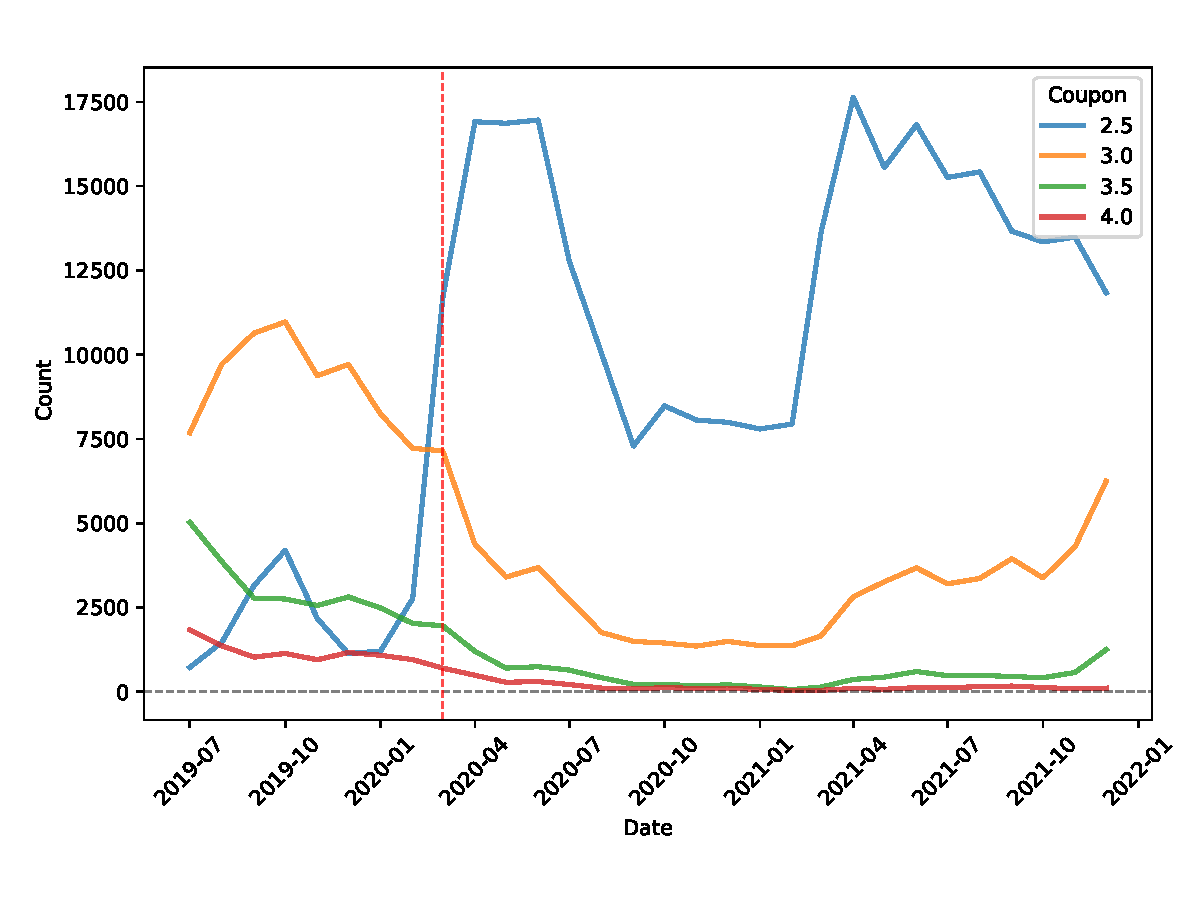
\includegraphics[width=0.998\textwidth]{../results/figures/winner_bid_count_mat30_loan1_timeseries_cpmonthly_2.5_4_.pdf}
      \caption{ Number of auctions}
     \end{subfigure}
     \begin{subfigure}[b]{0.49\textwidth}
      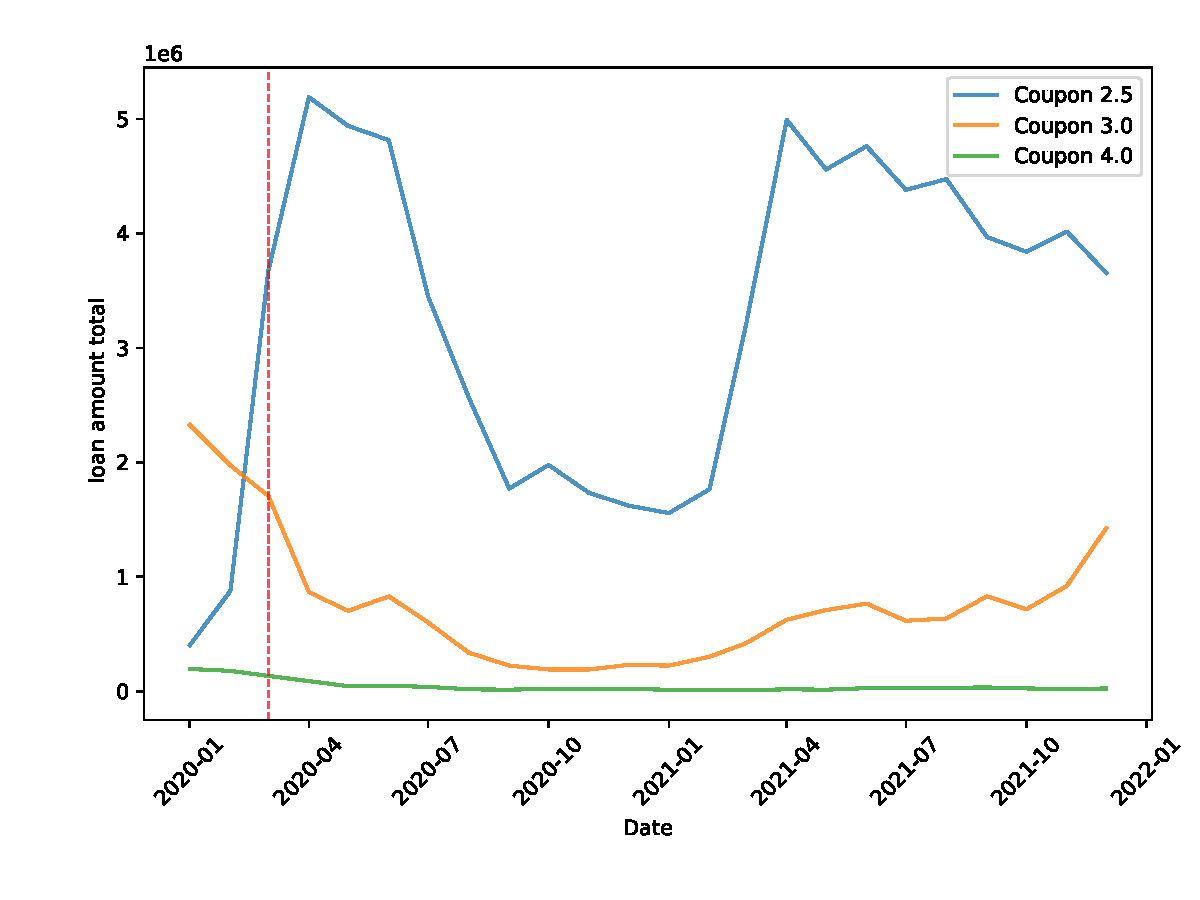
\includegraphics[width=0.998\textwidth]{../results/figures/LoanAmount_sum_mat30_loan1_timeseries_cpmonthly_2.5_4_.pdf}
      \caption{Loan amount}
     \end{subfigure}
     \begin{subfigure}[b]{0.49\textwidth}
      \includegraphics[width=0.998\textwidth]{../results/figures/w_winner_bid_mean_mat30_loan1_timeseries_cpmonthly
      \caption{ Mean of highest net bid}
     \end{subfigure}
     \begin{subfigure}[b]{0.49\textwidth}
      \includegraphics[width=0.998\textwidth]{../results/figures/winner_bid_median_mat30_loan1_timeseries_cp_monthly_2.5_4_.pdf}
      \caption{ Median of highest net bid}
     \end{subfigure}
   \caption{OB auction outcomes. } 
   \begin{minipage}{\textwidth}
      \footnotesize{\textit{Notes:} The figure shows the time series of auction outcomes for Conforming loans with a 30-year maturity.  The vertical lines is March 1. For reference, Bloomberg TBA prices are aggregated for all forward months and coupons between 1 and 7. }
      \end{minipage}
\end{figure}

\pagebreak
% \subsubsection{Comparison of note rates}

% \begin{figure}[h]
%   \centering
%   \begin{subfigure}[b]{0.49\textwidth}
%       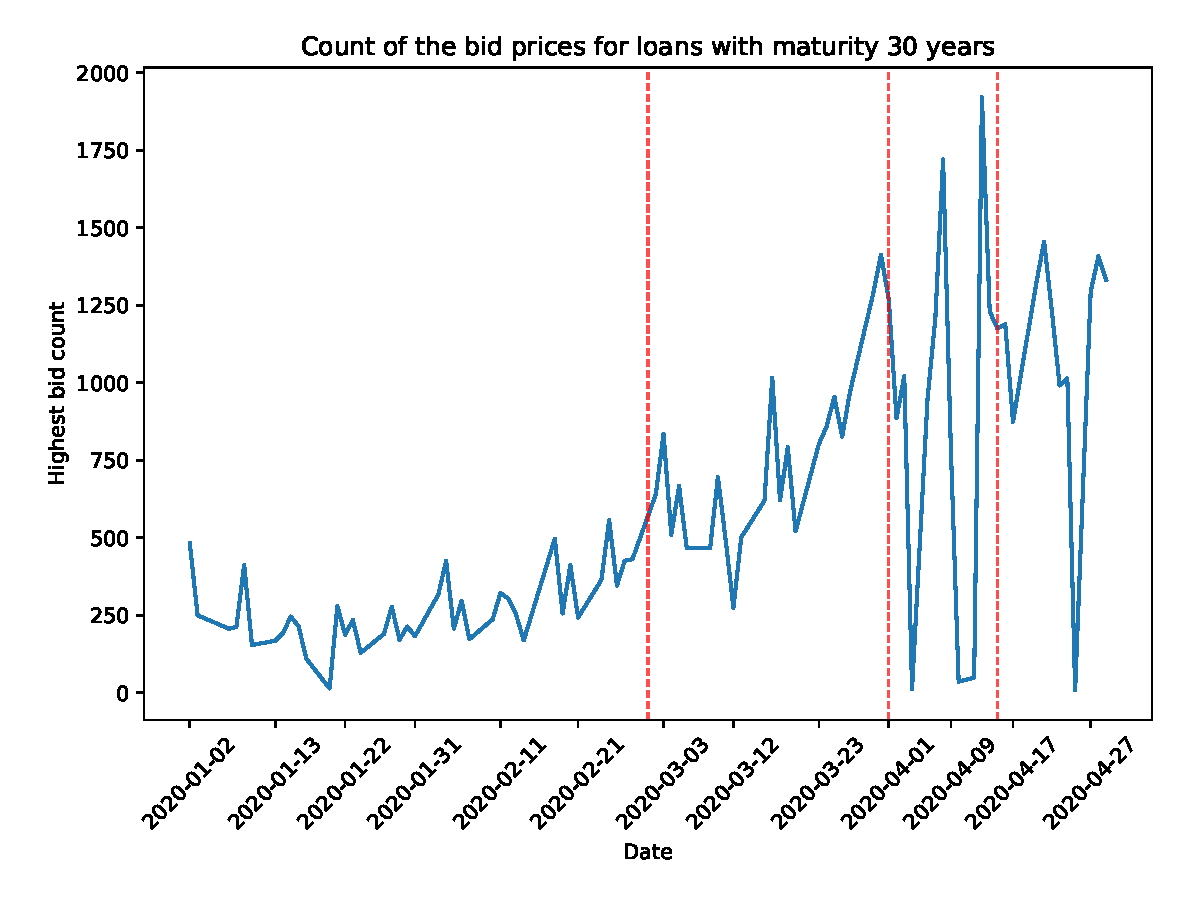
\includegraphics[width=0.998\textwidth]{../results/figures/winner_bid_count_mat30_loan1_timeseries_nr_3_3.75.pdf}
%       \caption{ Number of auctions}
%      \end{subfigure}
%      \begin{subfigure}[b]{0.49\textwidth}
%       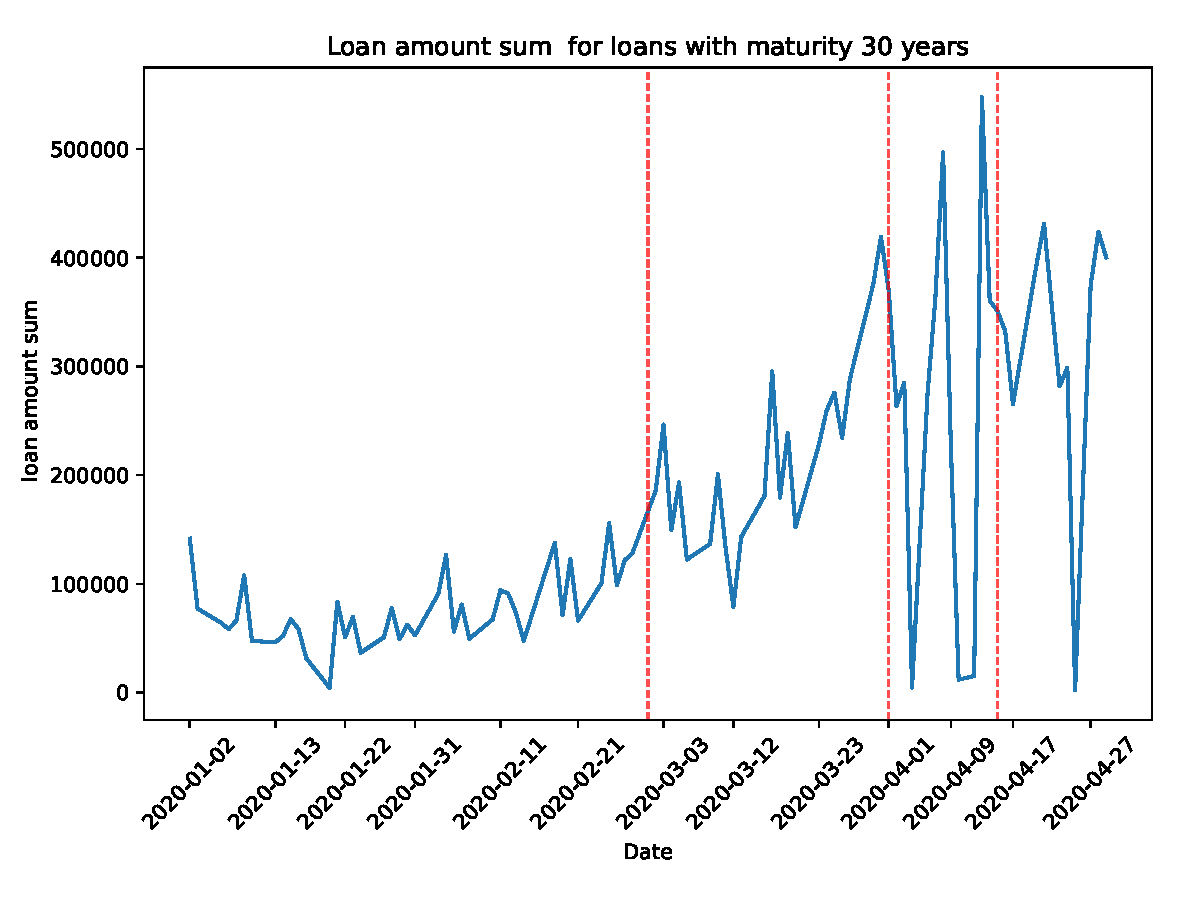
\includegraphics[width=0.998\textwidth]{../results/figures/LoanAmount_sum_mat30_loan1_timeseries_nr_3_3.75.pdf}
%       \caption{ Daily loan amount}
%      \end{subfigure}
%      \begin{subfigure}[b]{0.49\textwidth}
%       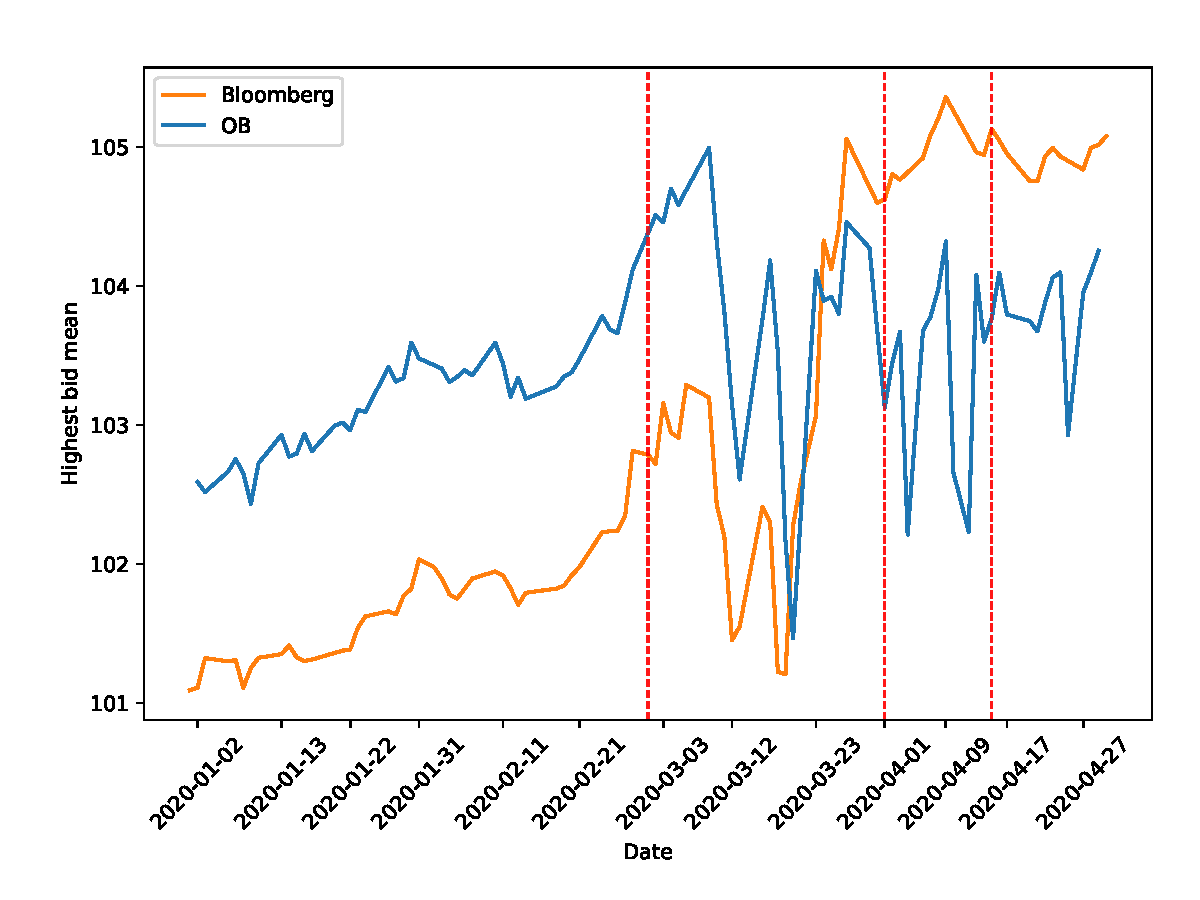
\includegraphics[width=0.998\textwidth]{../results/figures/w_winner_bid_mean_mat30_loan1_timeseries_nr_3_3.75.pdf}
%       \caption{ Weighted mean of highest bid}
%      \end{subfigure}
%      \begin{subfigure}[b]{0.49\textwidth}
%       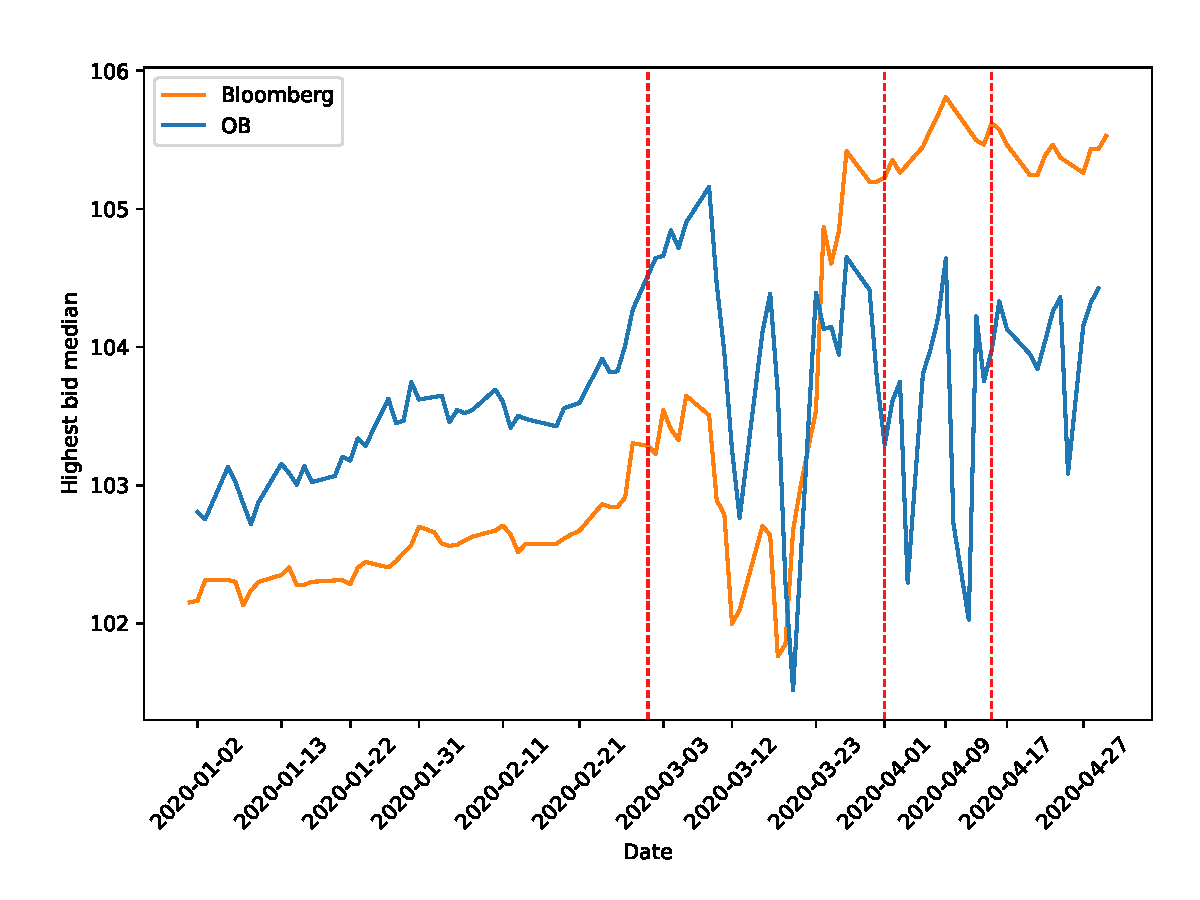
\includegraphics[width=0.998\textwidth]{../results/figures/winner_bid_median_mat30_loan1_timeseries_nr_3_3.75.pdf}
%       \caption{ Median of highest bid}
%      \end{subfigure}
%    \caption{OB auction outcomes for note rates between 3\% and 3.75\%}
%    \begin{minipage}{\textwidth}
%       \footnotesize{\textit{Notes:} The figure shows time series of auction outcomes for Conforming loans with a 30-year maturity. The vertical lines is March 1. For reference, Bloomberg TBA prices are aggregated for all forward months and coupons between 2.5, 3, and 3.5. } 
%       \end{minipage}
% \end{figure}

% \pagebreak

% \begin{figure}[h]
%   \centering
%   \begin{subfigure}[b]{0.49\textwidth}
%       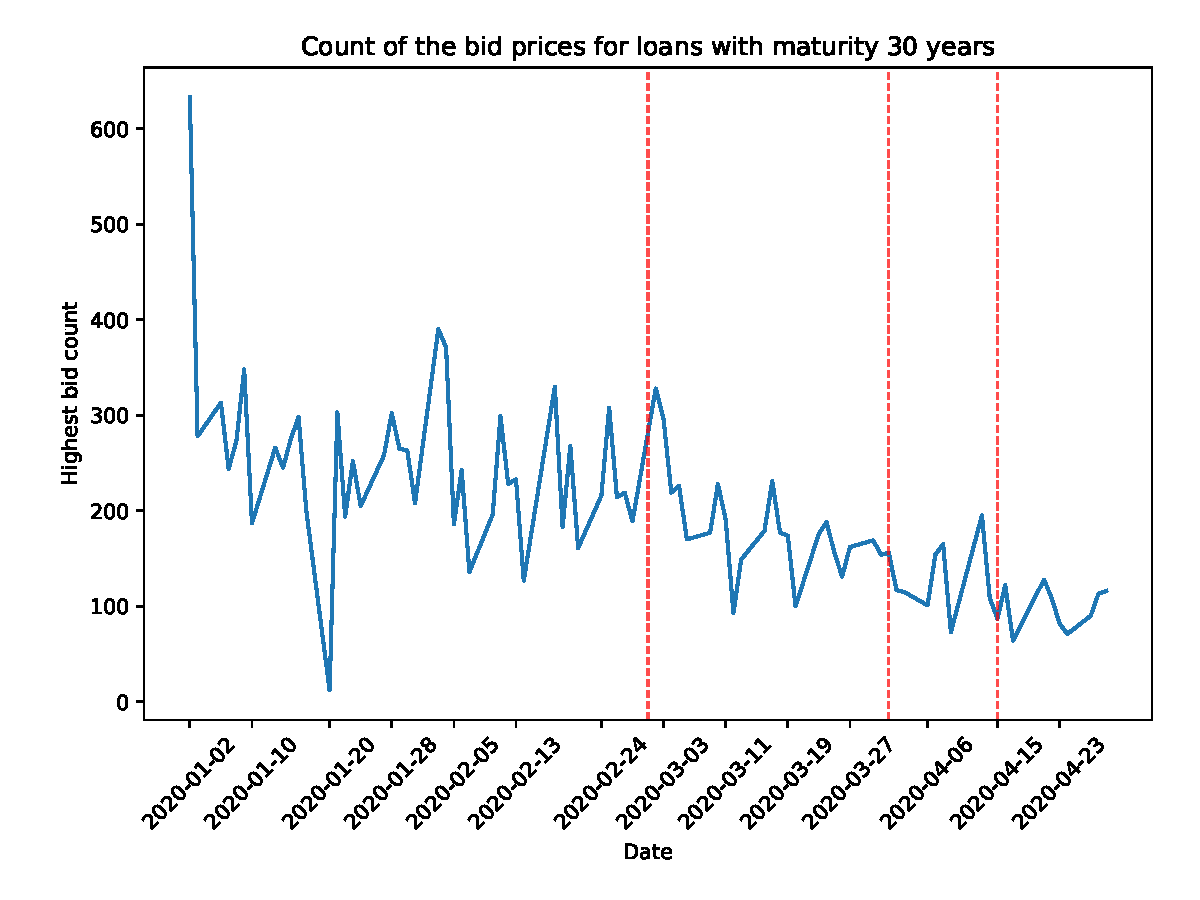
\includegraphics[width=0.998\textwidth]{../results/figures/winner_bid_count_mat30_loan1_timeseries_nr_4_4.75.pdf}
%       \caption{ Number of auctions}
%      \end{subfigure}
%      \begin{subfigure}[b]{0.49\textwidth}
%       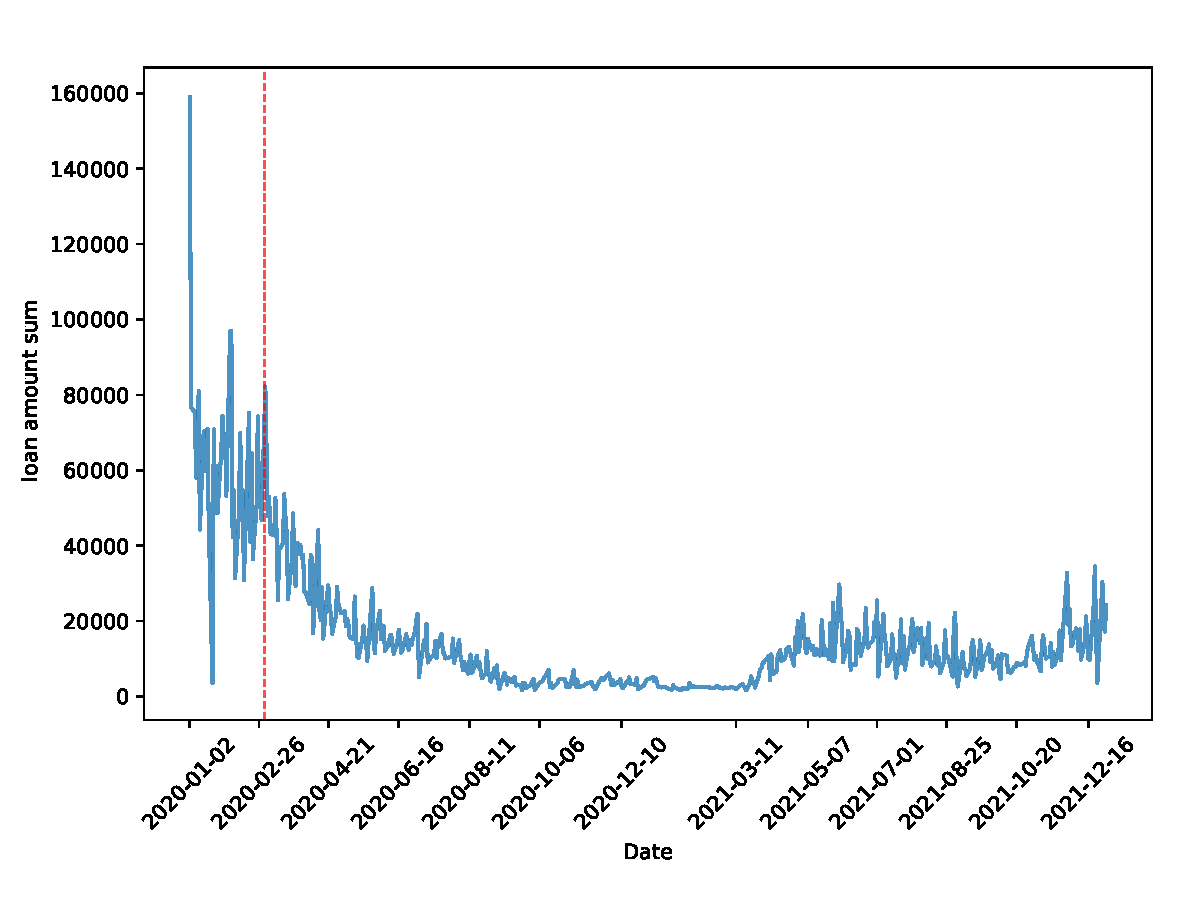
\includegraphics[width=0.998\textwidth]{../results/figures/LoanAmount_sum_mat30_loan1_timeseries_nr_4_4.75.pdf}
%       \caption{ Daily loan amount}
%      \end{subfigure}
%      \begin{subfigure}[b]{0.49\textwidth}
%       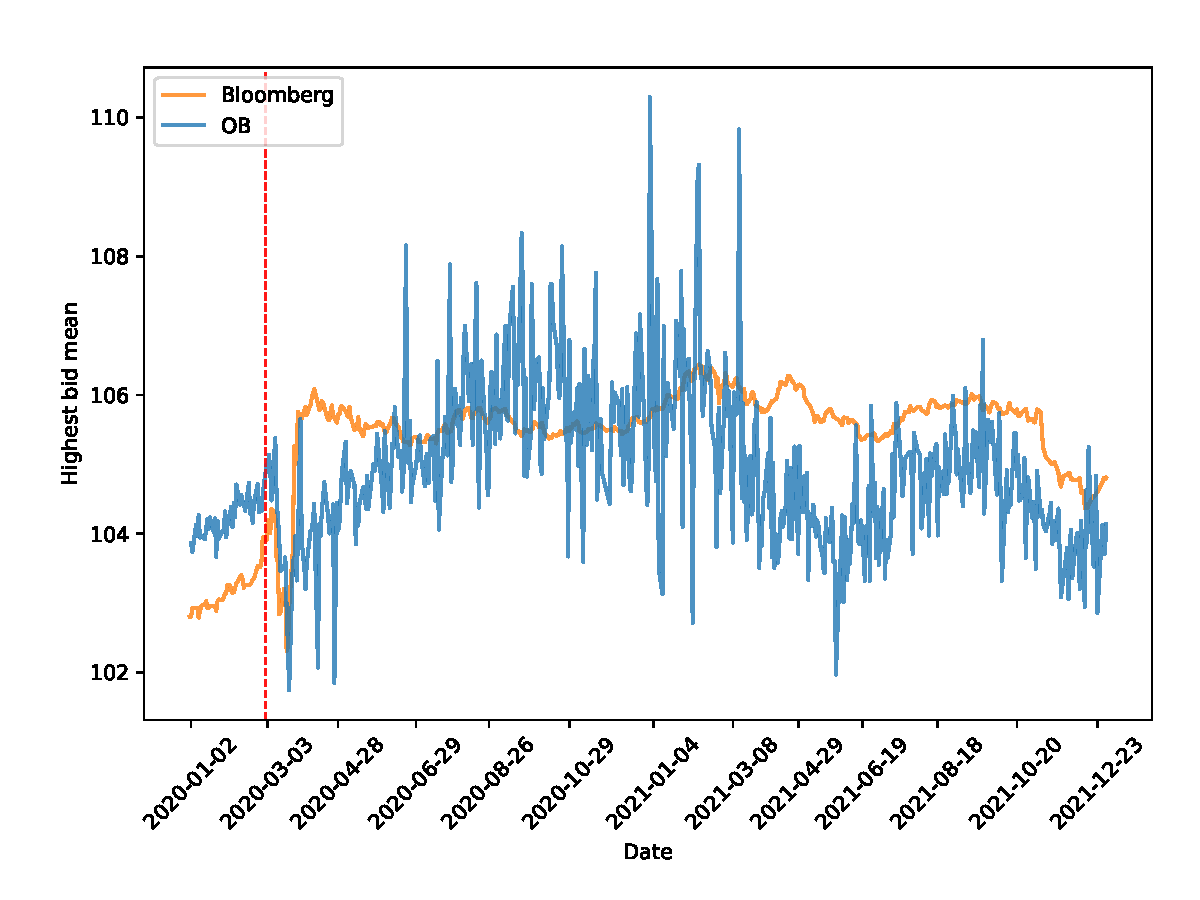
\includegraphics[width=0.998\textwidth]{../results/figures/w_winner_bid_mean_mat30_loan1_timeseries_nr_4_4.75.pdf}
%       \caption{ Weighted mean of highest bid}
%      \end{subfigure}
%      \begin{subfigure}[b]{0.49\textwidth}
%       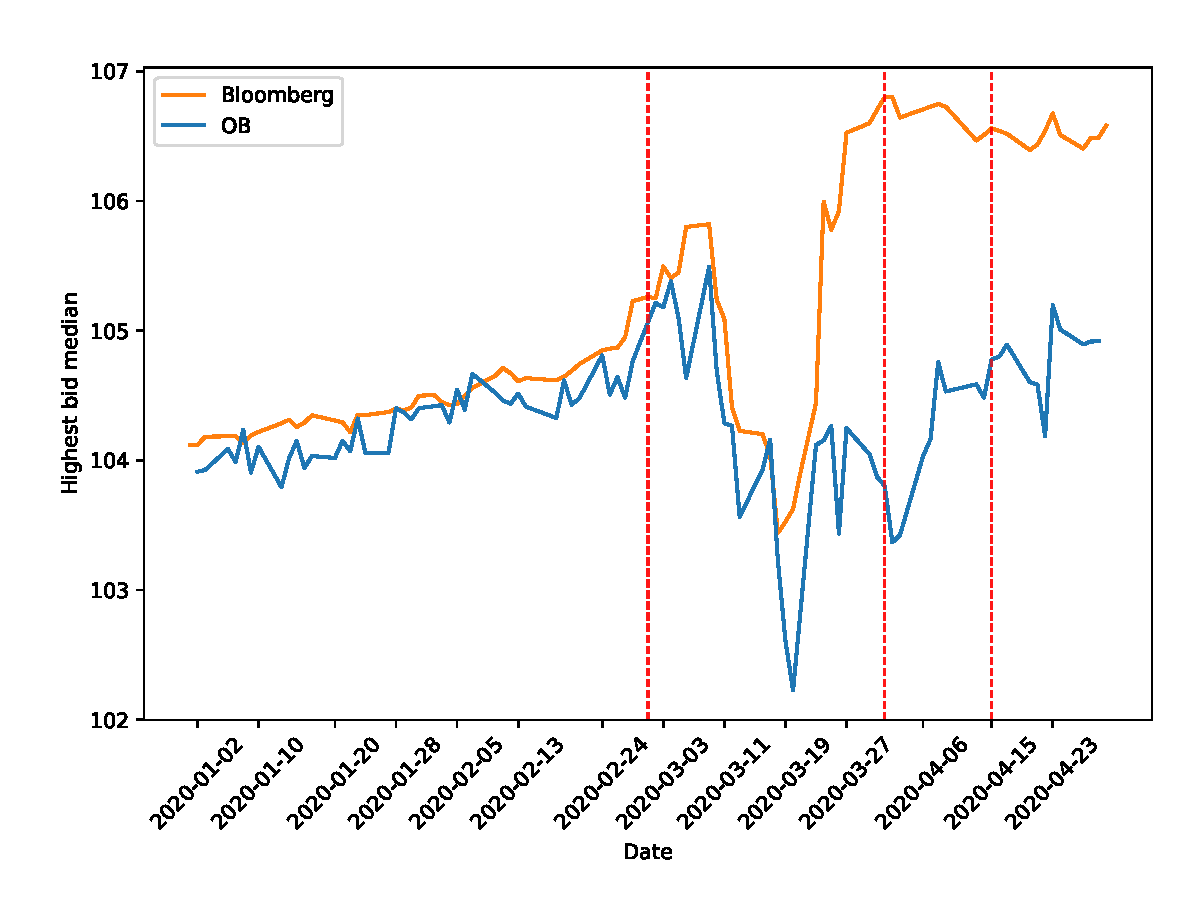
\includegraphics[width=0.998\textwidth]{../results/figures/winner_bid_median_mat30_loan1_timeseries_nr_4_4.75.pdf}
%       \caption{ Median of highest bid}
%      \end{subfigure}
%    \caption{OB auction outcomes for note rates between 4\% and 4.75\%}
%    \begin{minipage}{\textwidth}
%       \footnotesize{\textit{Notes:} The figure shows the time series of auction outcomes for Conforming loans with a 30-year maturity.  The vertical lines is March 1. For reference, Bloomberg TBA prices are aggregated for all forward months and coupons 3.5, 4, and 4.5. } 
%       \end{minipage}
% \end{figure}

\pagebreak

\subsection{Distress signs in the OB auctions}

Below, we show distress and illiquidity measures in the OB auctions during the early Covid period. The variables are defined as follows:
\begin{itemize}
\item \textbf{Days to auction}: Number of days between the auction date and the date the loan originated.
\item \textbf{Number of participants}: Number of participants in the auction.
\item  \textbf{Sell rate:} Rate to which the loan is sold to an auction participant. 
\item \textbf{Fraction of bulk bidders:} Fraction of bids that are bulk bids.
\end{itemize}
\begin{figure}[h]
  \centering
  \begin{subfigure}[b]{0.49\textwidth}
      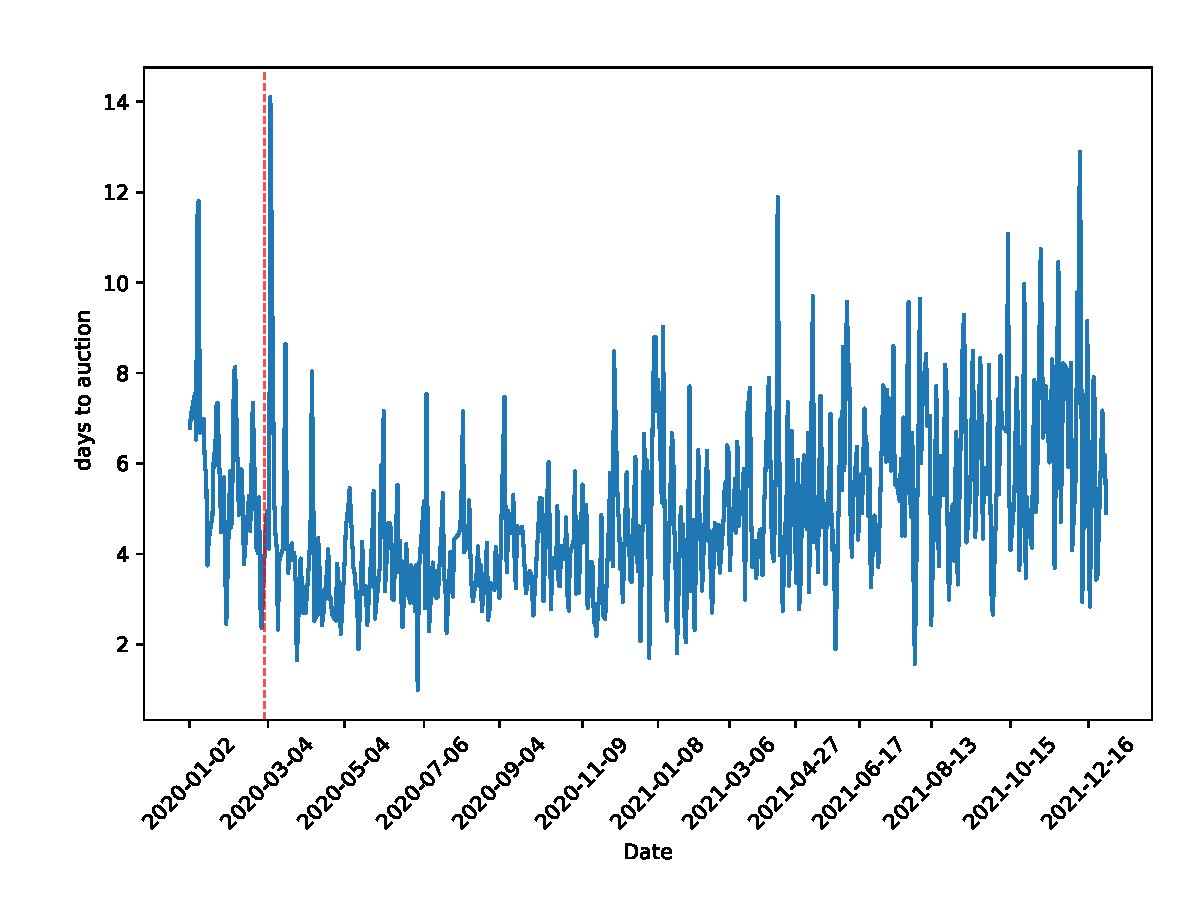
\includegraphics[width=0.998\textwidth]{../results/figures/DaysToAuction_mean_mat30_loan1_timeseries_nr_1_7.pdf}
      \caption{Days to auction}
     \end{subfigure}
     \begin{subfigure}[b]{0.49\textwidth}
      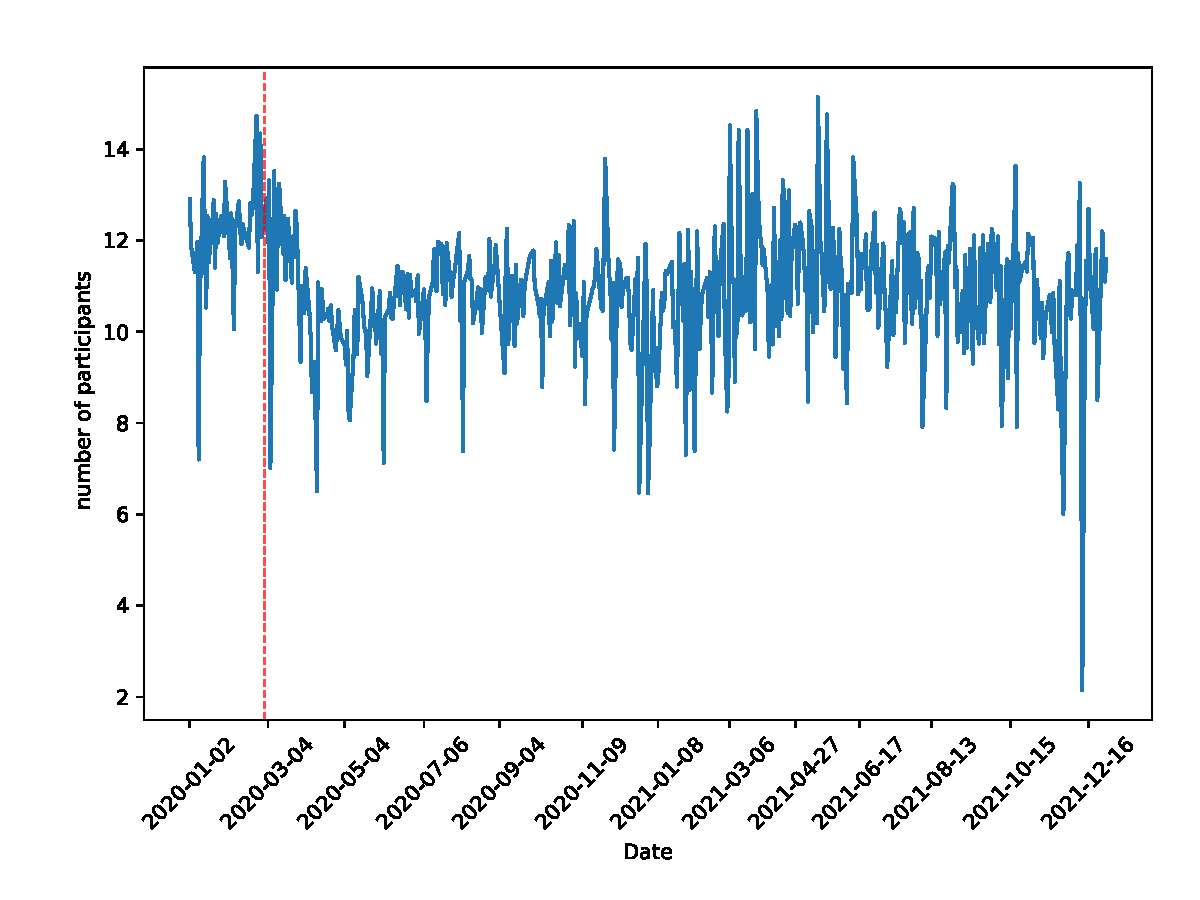
\includegraphics[width=0.998\textwidth]{../results/figures/Number of Participants_mean_mat30_loan1_timeseries_nr_1_7.pdf}
      \caption{ Number of participants}
     \end{subfigure}
     \begin{subfigure}[b]{0.49\textwidth}
      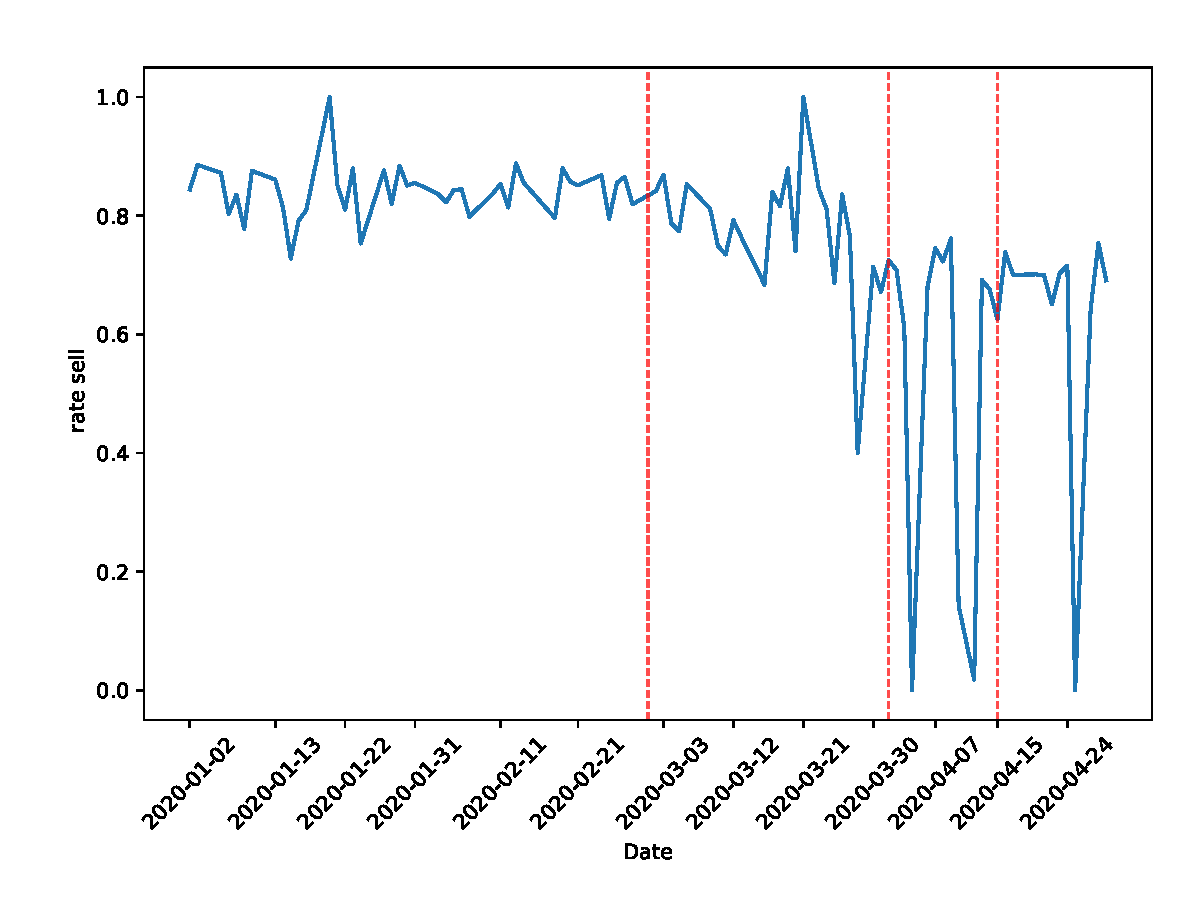
\includegraphics[width=0.998\textwidth]{../results/figures/dummy_sell_any_mean_mat30_loan1_timeseries_nr_1_7.pdf}
      \caption{ Sell rate}
     \end{subfigure}
     \begin{subfigure}[b]{0.49\textwidth}
      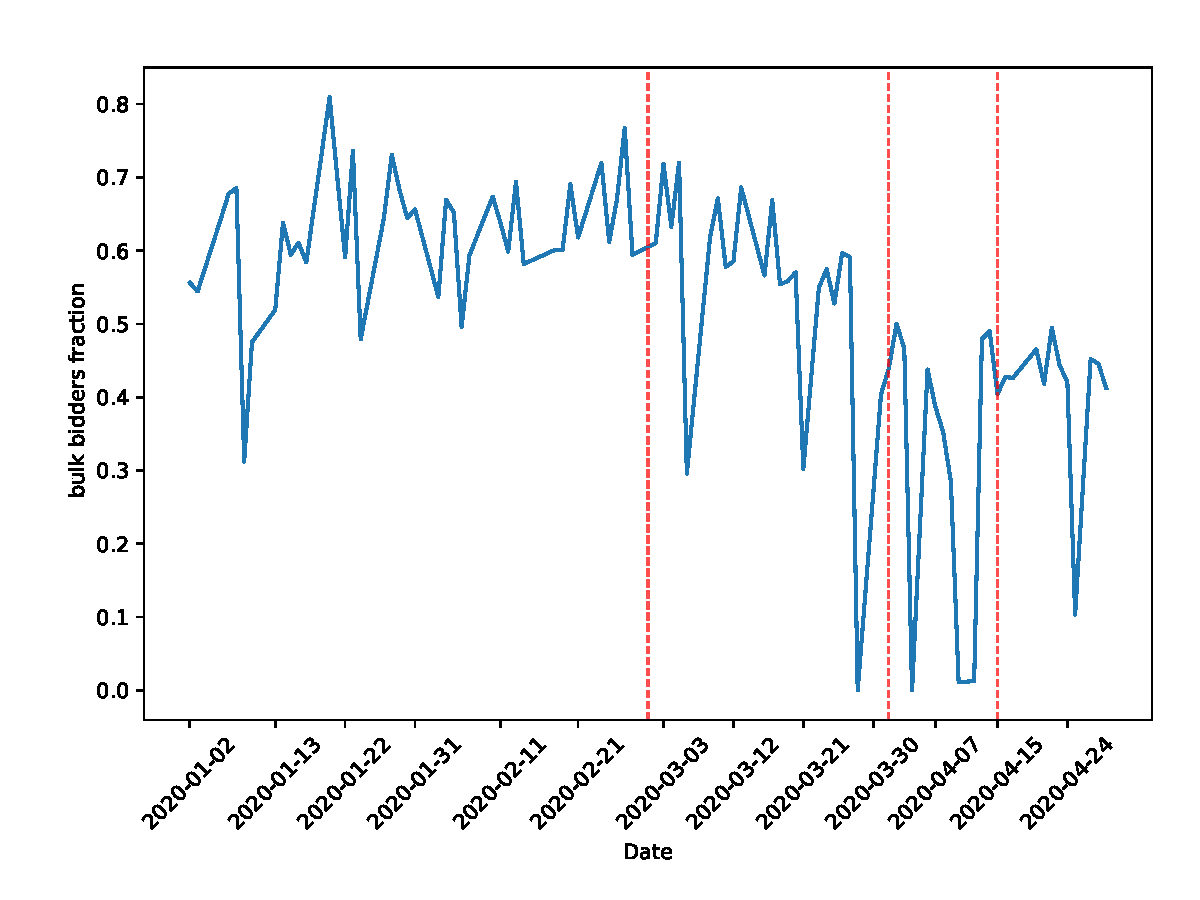
\includegraphics[width=0.998\textwidth]{../results/figures/bulk_bidders_fraction_mean_mat30_loan1_timeseries_nr_1_7.pdf}
      \caption{ Fraction of bulk bidders}
     \end{subfigure}
     \caption{OB auction outcomes. } 
   \begin{minipage}{\textwidth}
      \footnotesize{\textit{Notes:} The figure shows time series of auction outcomes for Conforming loans with a 30-year maturity. The vertical lines is March 1.  } 
      \end{minipage}
\end{figure}

\pagebreak
\subsubsection{Comparison of note rates}

Below, we show the same variables as above, but for different note rates. 

\begin{figure}[h]
  \centering
  \begin{subfigure}[b]{0.49\textwidth}
      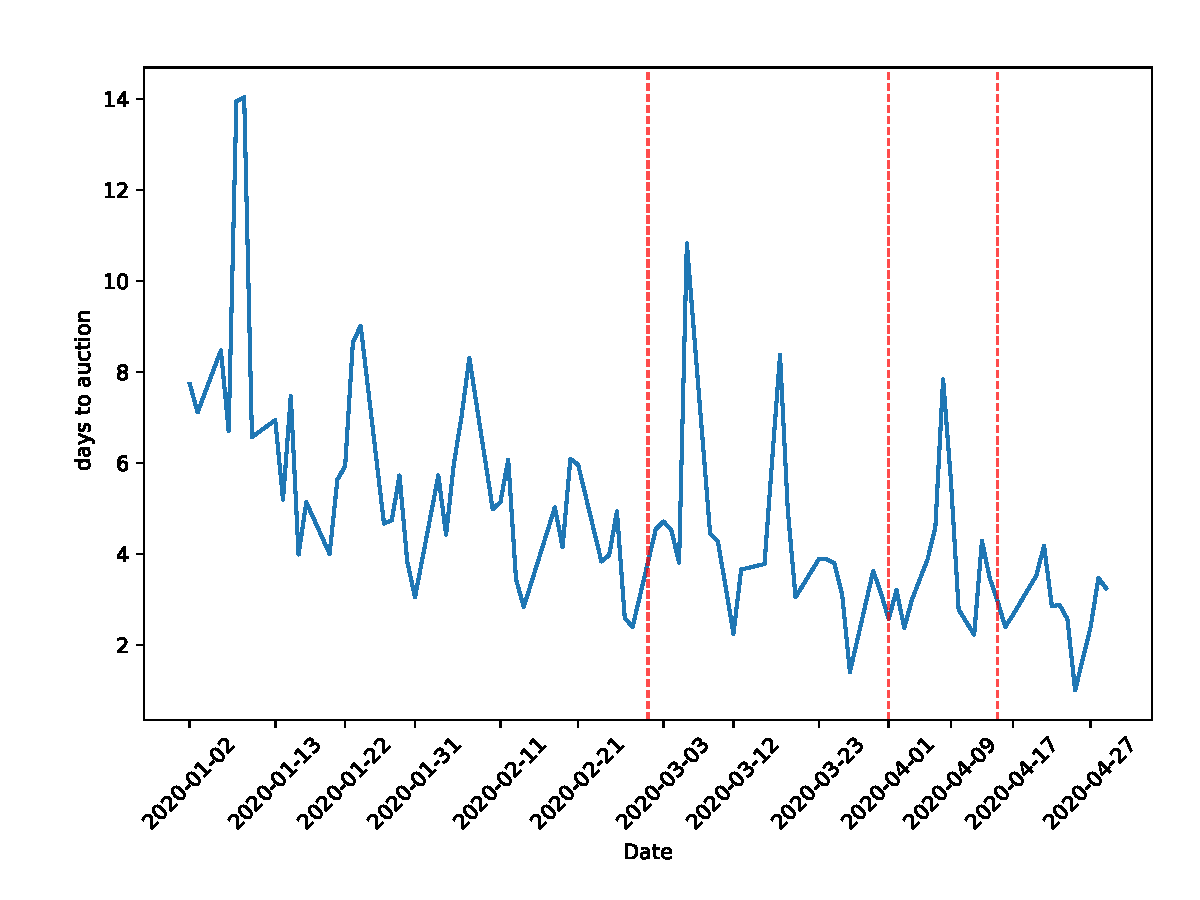
\includegraphics[width=0.998\textwidth]{../results/figures/DaysToAuction_mean_mat30_loan1_timeseries_nr_3_3.75.pdf}
      \caption{Days to auction}
     \end{subfigure}
     \begin{subfigure}[b]{0.49\textwidth}
      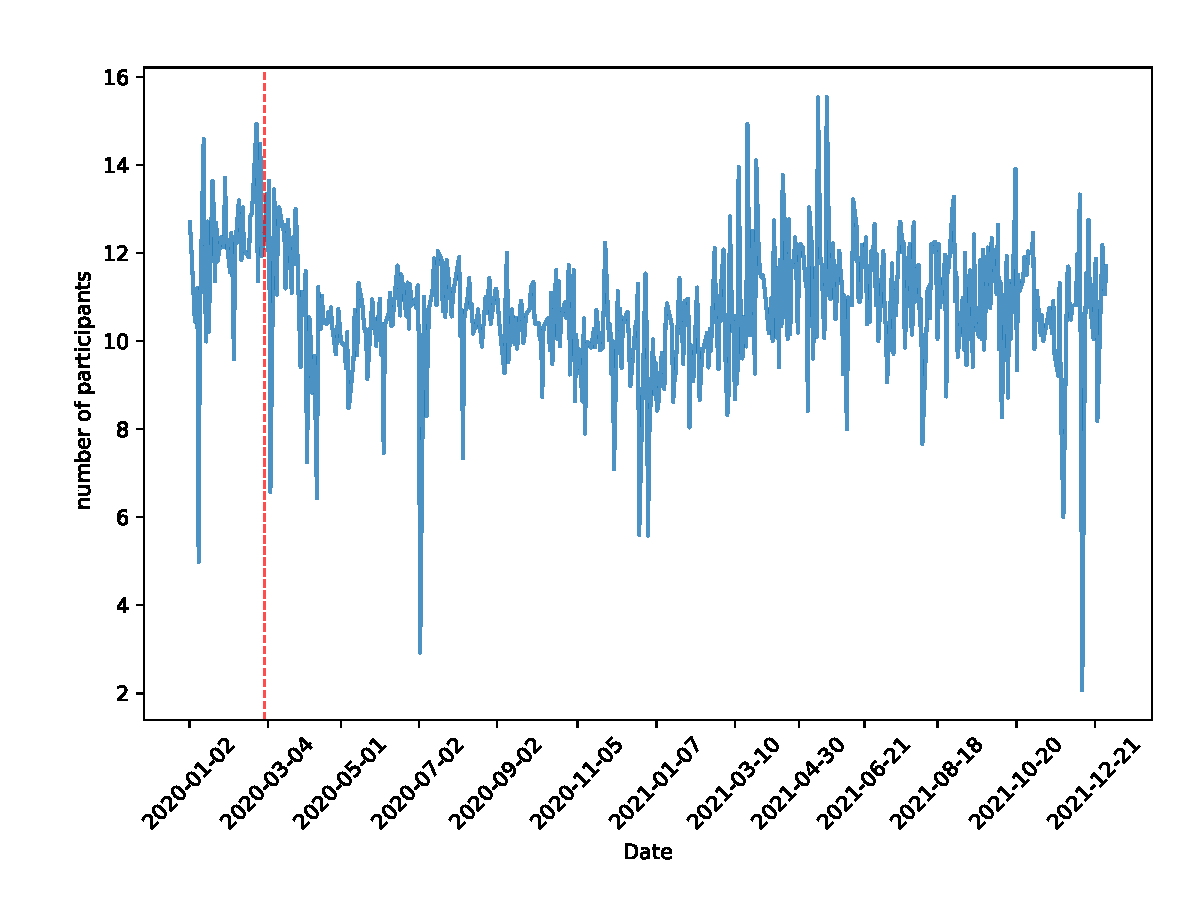
\includegraphics[width=0.998\textwidth]{../results/figures/Number of Participants_mean_mat30_loan1_timeseries_nr_3_3.75.pdf}
      \caption{ Number of participants}
     \end{subfigure}
     \begin{subfigure}[b]{0.49\textwidth}
      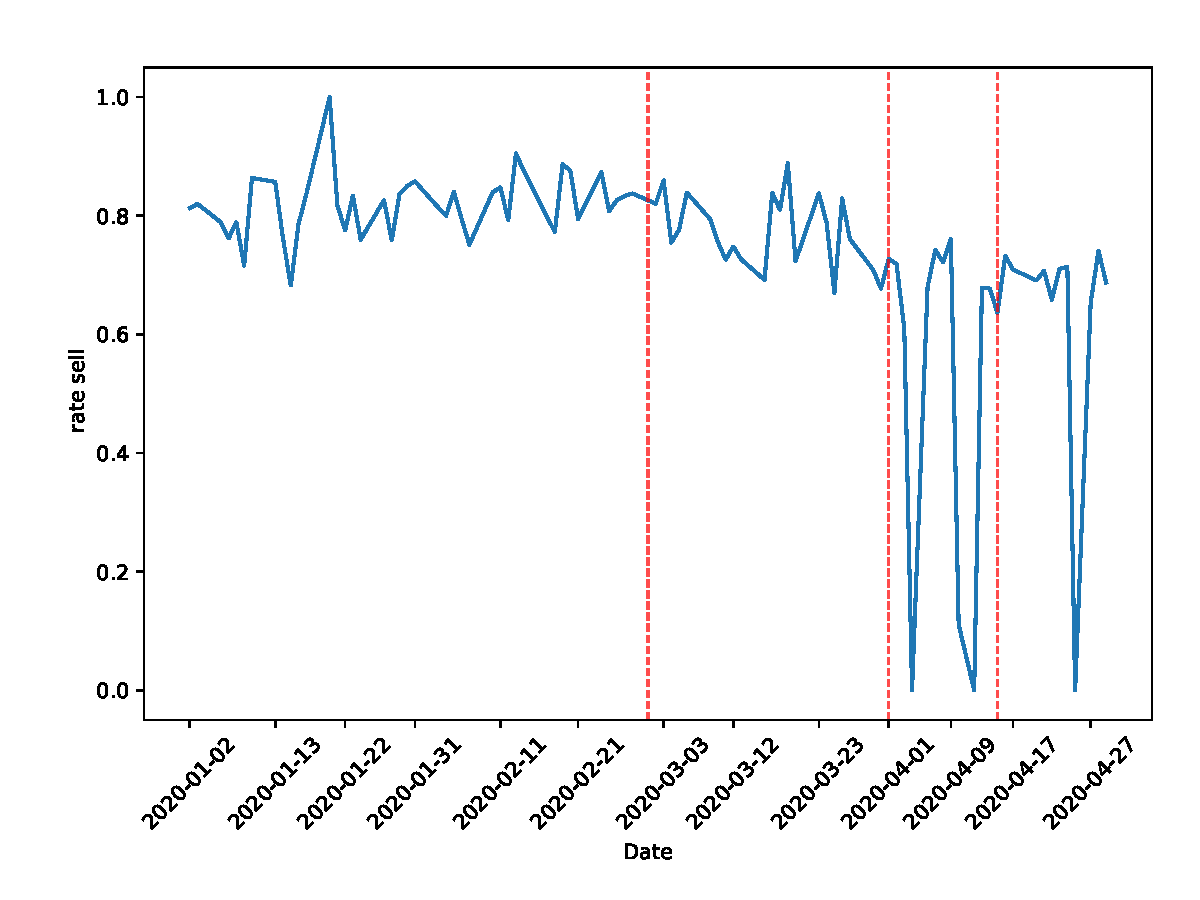
\includegraphics[width=0.998\textwidth]{../results/figures/dummy_sell_any_mean_mat30_loan1_timeseries_nr_3_3.75.pdf}
      \caption{ Sell rate}
     \end{subfigure}
     \begin{subfigure}[b]{0.49\textwidth}
      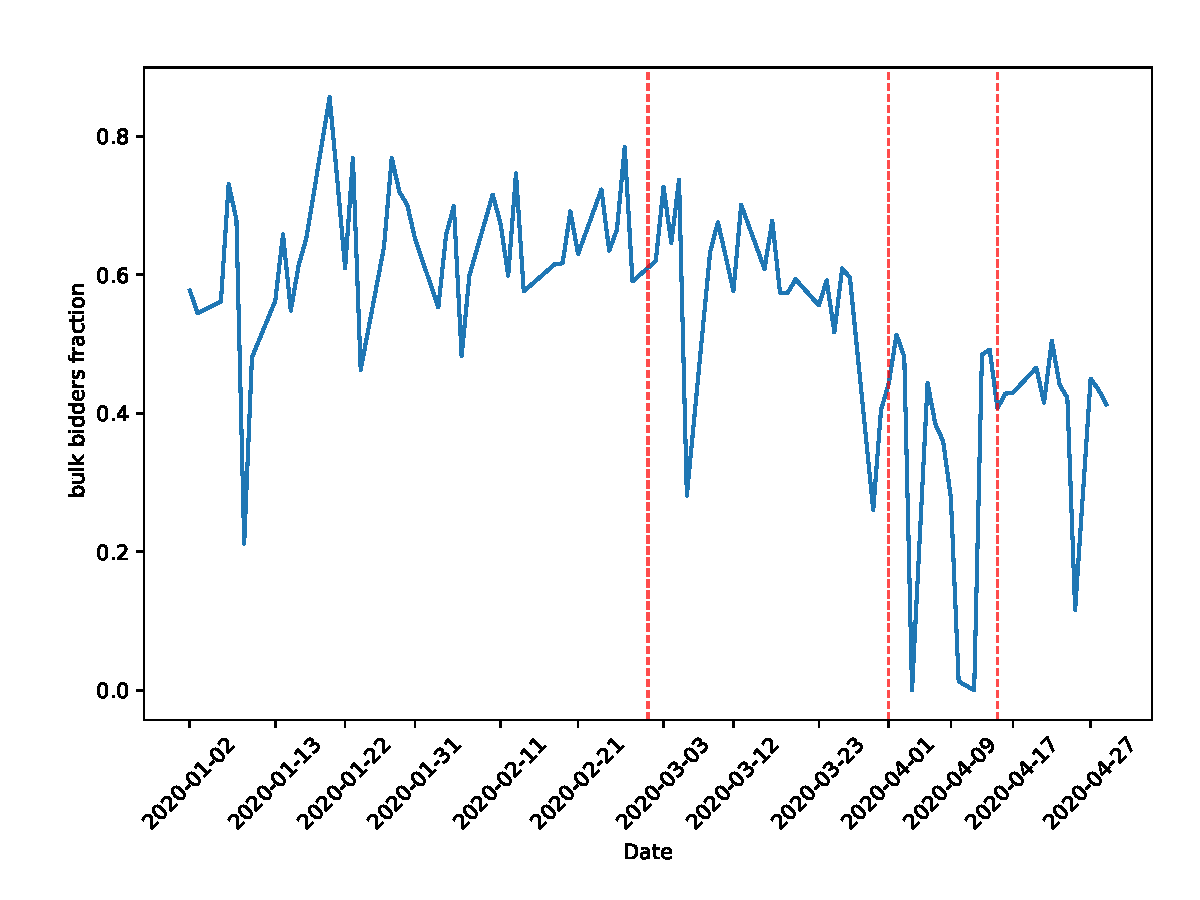
\includegraphics[width=0.998\textwidth]{../results/figures/bulk_bidders_fraction_mean_mat30_loan1_timeseries_nr_3_3.75.pdf}
      \caption{ Fraction of bulk bidders}
     \end{subfigure}
     \caption{OB auction outcomes for note rates between 3\% and 3.75\%.  } 
   \begin{minipage}{\textwidth}
      \footnotesize{\textit{Notes:} The figure shows time series of auction outcomes for Conforming loans with a 30-year maturity. The vertical lines is March 1.  } 
      \end{minipage}
\end{figure}

\pagebreak
\begin{figure}[h]
  \centering
  \begin{subfigure}[b]{0.49\textwidth}
      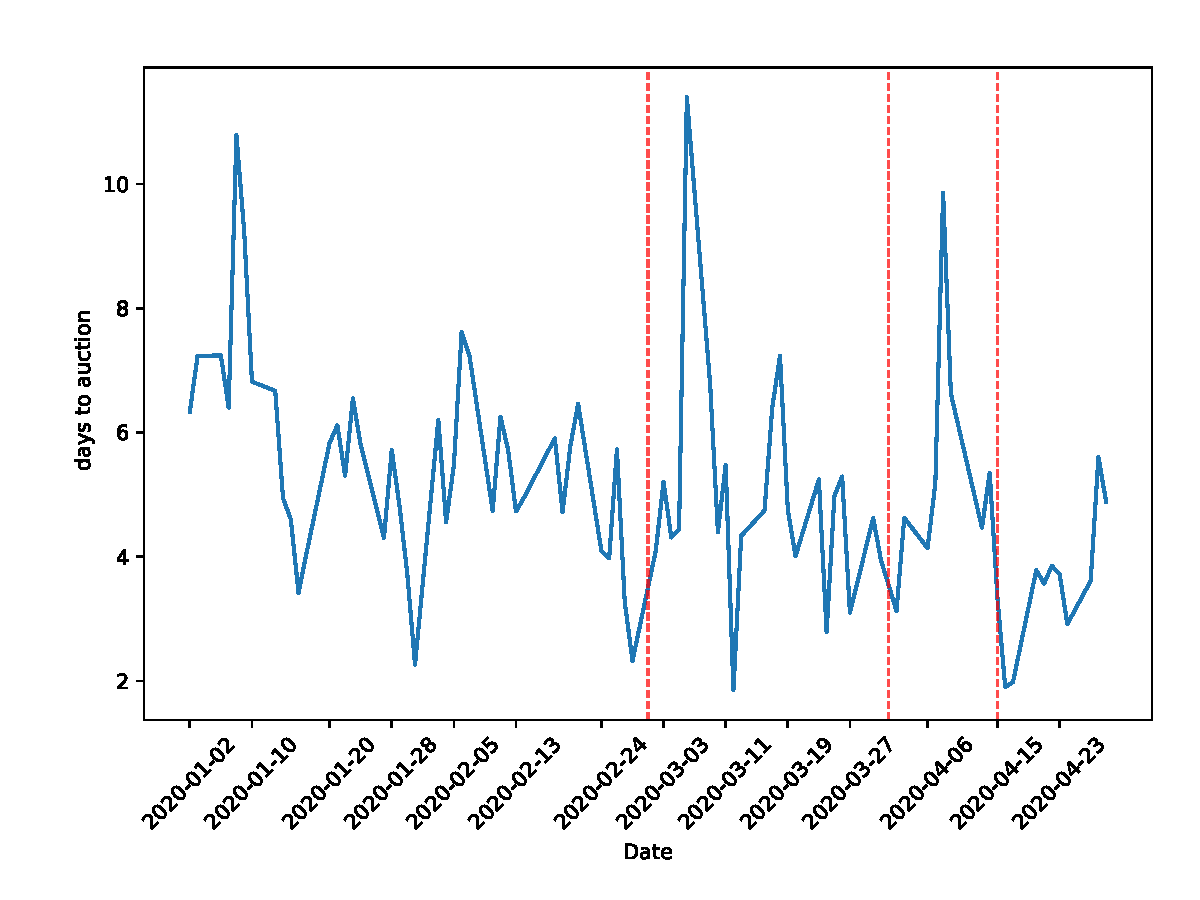
\includegraphics[width=0.998\textwidth]{../results/figures/DaysToAuction_mean_mat30_loan1_timeseries_nr_4_4.75.pdf}
      \caption{Days to auction}
     \end{subfigure}
     \begin{subfigure}[b]{0.49\textwidth}
      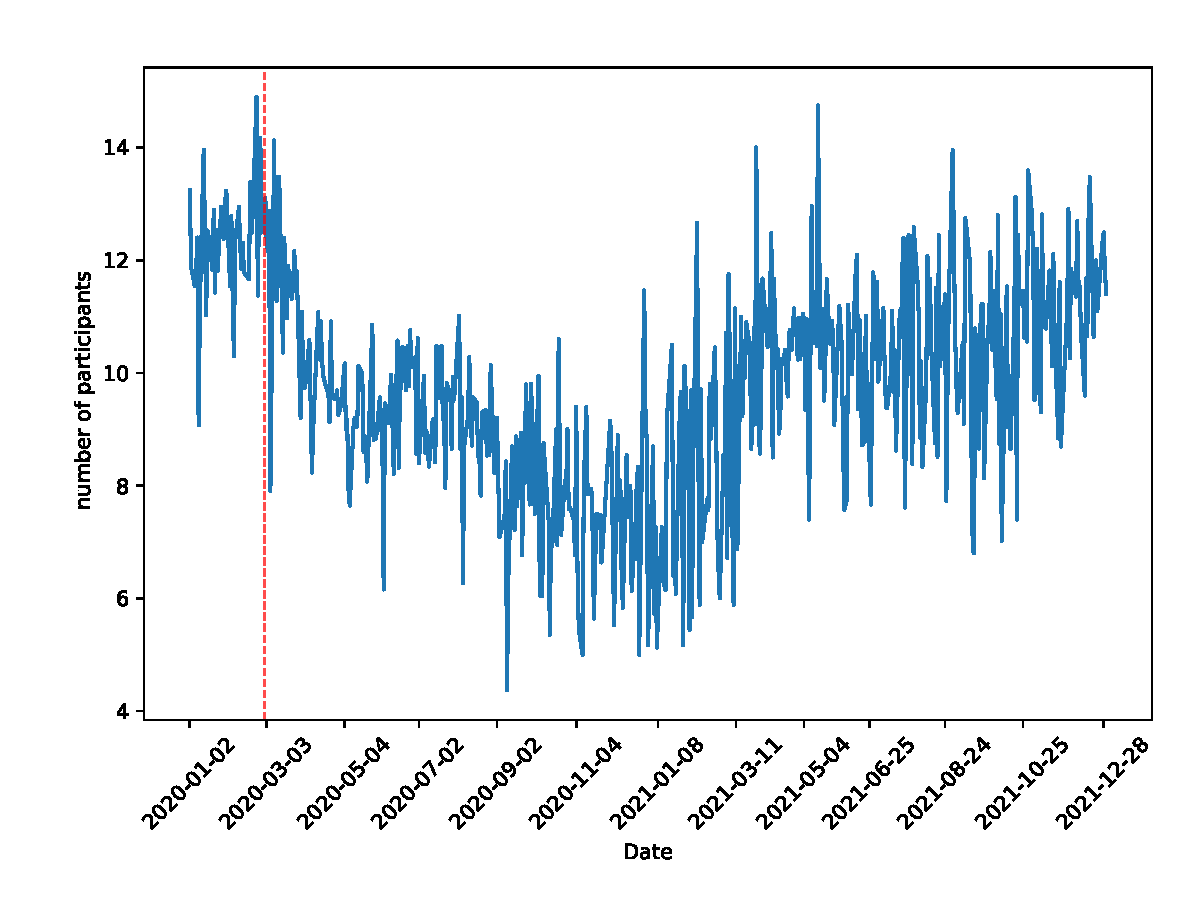
\includegraphics[width=0.998\textwidth]{../results/figures/Number of Participants_mean_mat30_loan1_timeseries_nr_4_4.75.pdf}
      \caption{ Number of participants}
     \end{subfigure}
     \begin{subfigure}[b]{0.49\textwidth}
      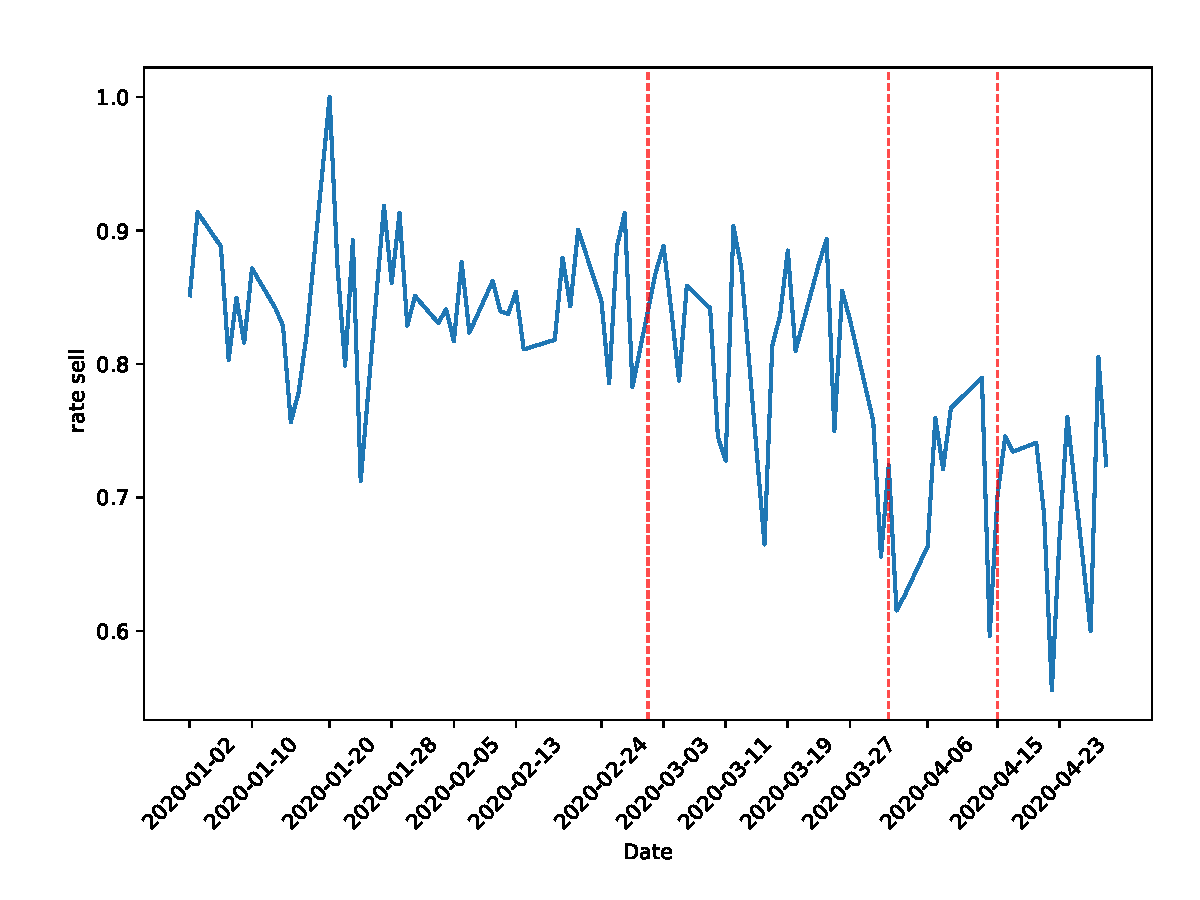
\includegraphics[width=0.998\textwidth]{../results/figures/dummy_sell_any_mean_mat30_loan1_timeseries_nr_4_4.75.pdf}
      \caption{ Sell rate}
     \end{subfigure}
     \begin{subfigure}[b]{0.49\textwidth}
      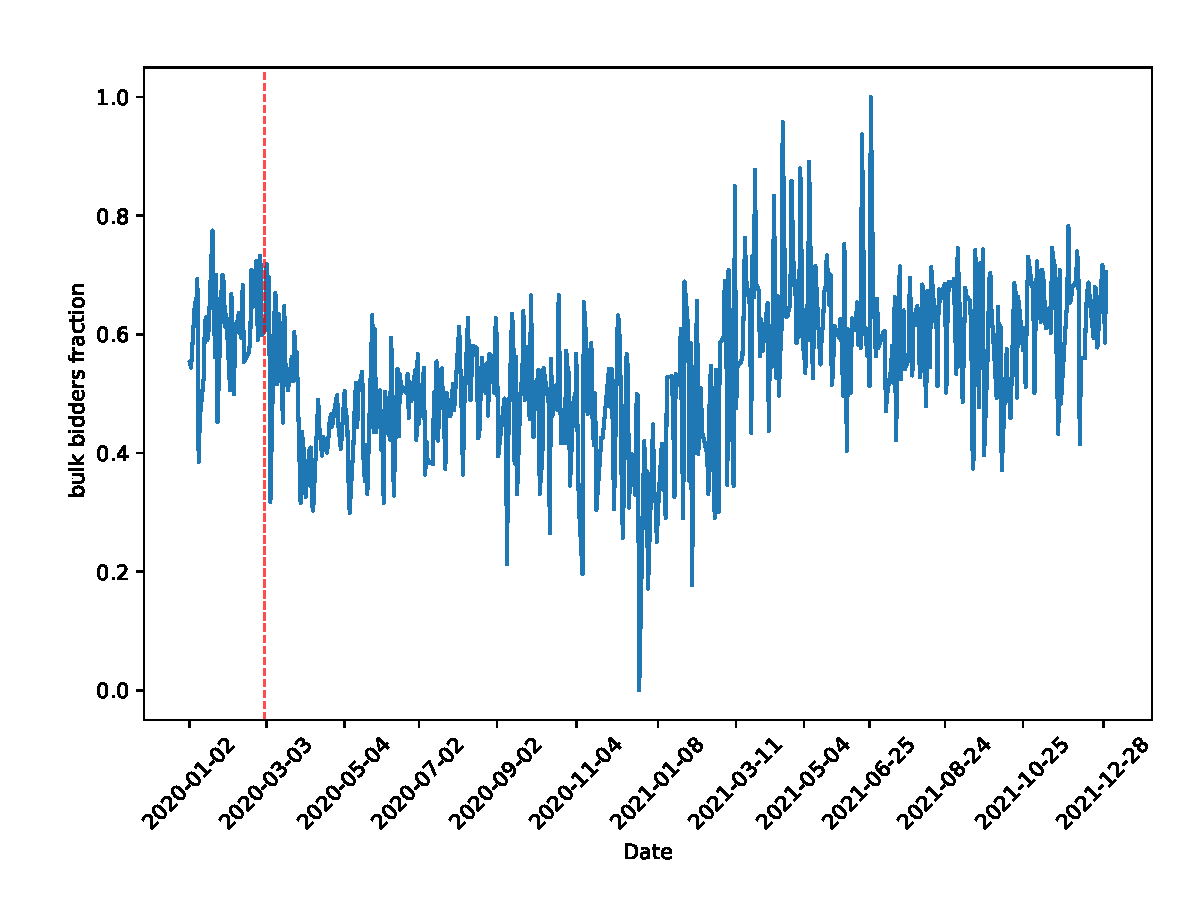
\includegraphics[width=0.998\textwidth]{../results/figures/bulk_bidders_fraction_mean_mat30_loan1_timeseries_nr_4_4.75.pdf}
      \caption{ Fraction of bulk bidders}
     \end{subfigure}
     \caption{OB auction outcomes for note rates between 4\% and 4.75\%. } 
   \begin{minipage}{\textwidth}
      \footnotesize{\textit{Notes:} The figure shows the time series of auction outcomes for Conforming loans with a 30-year maturity. The vertical lines is March 1.  } 
      \end{minipage}
\end{figure}


\pagebreak
\subsection{GSE response }

 In this section, we show the GSE response to the covid crisis. The variables are defined as follows:
\begin{itemize}
\item \textbf{Number of Enterprise Bids}: Number of bids per auction submitted by the GSEs (Fannie and Freddie).
\item \textbf{Fraction of loans sold to GSE}: Fraction of loans sold to the GSEs.
\end{itemize}

\begin{figure}[h]
  \centering
  \begin{subfigure}[b]{0.49\textwidth}
      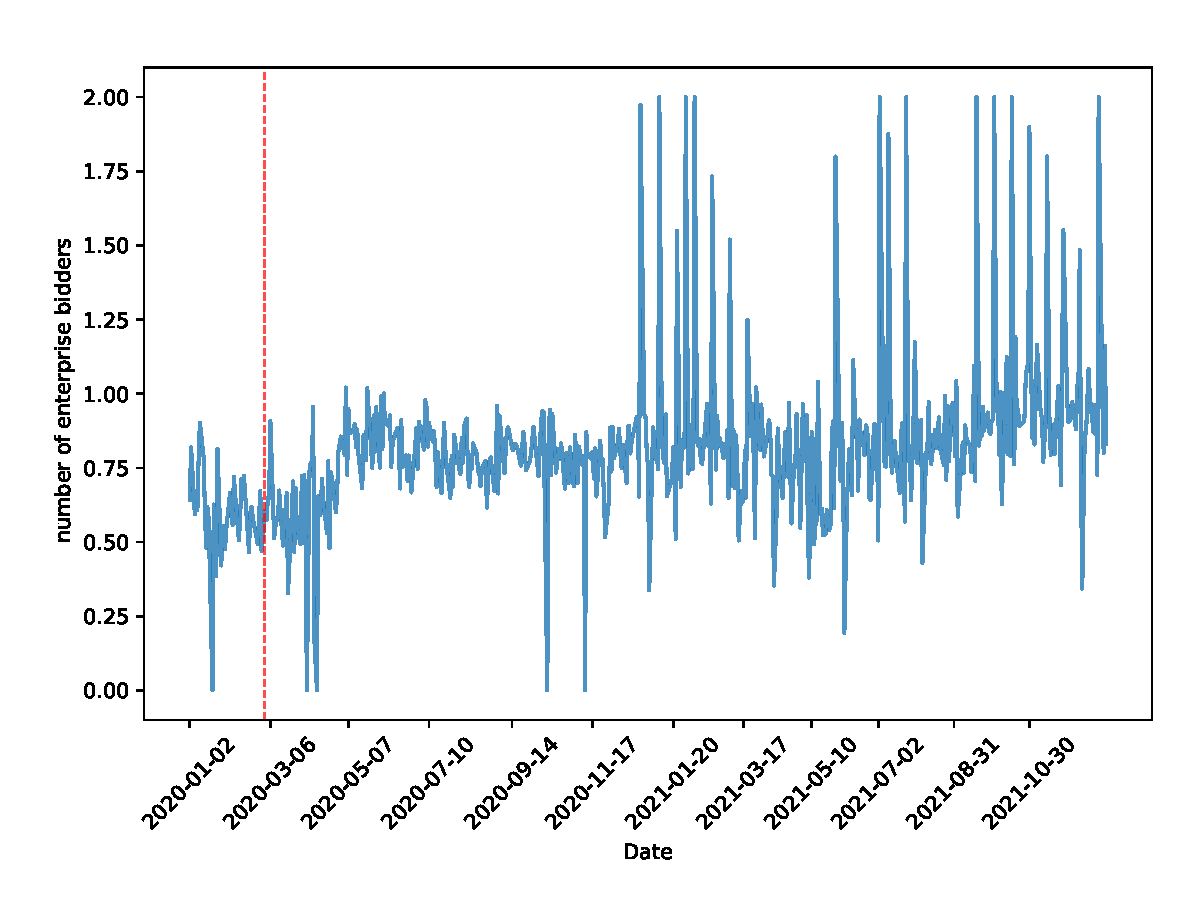
\includegraphics[width=0.998\textwidth]{../results/figures/Number of Enterprise Bidders_mean_mat30_loan1_timeseries_nr_1_7.pdf}
      \caption{Number of Enterprise Bids}
     \end{subfigure}
     \begin{subfigure}[b]{0.49\textwidth}
      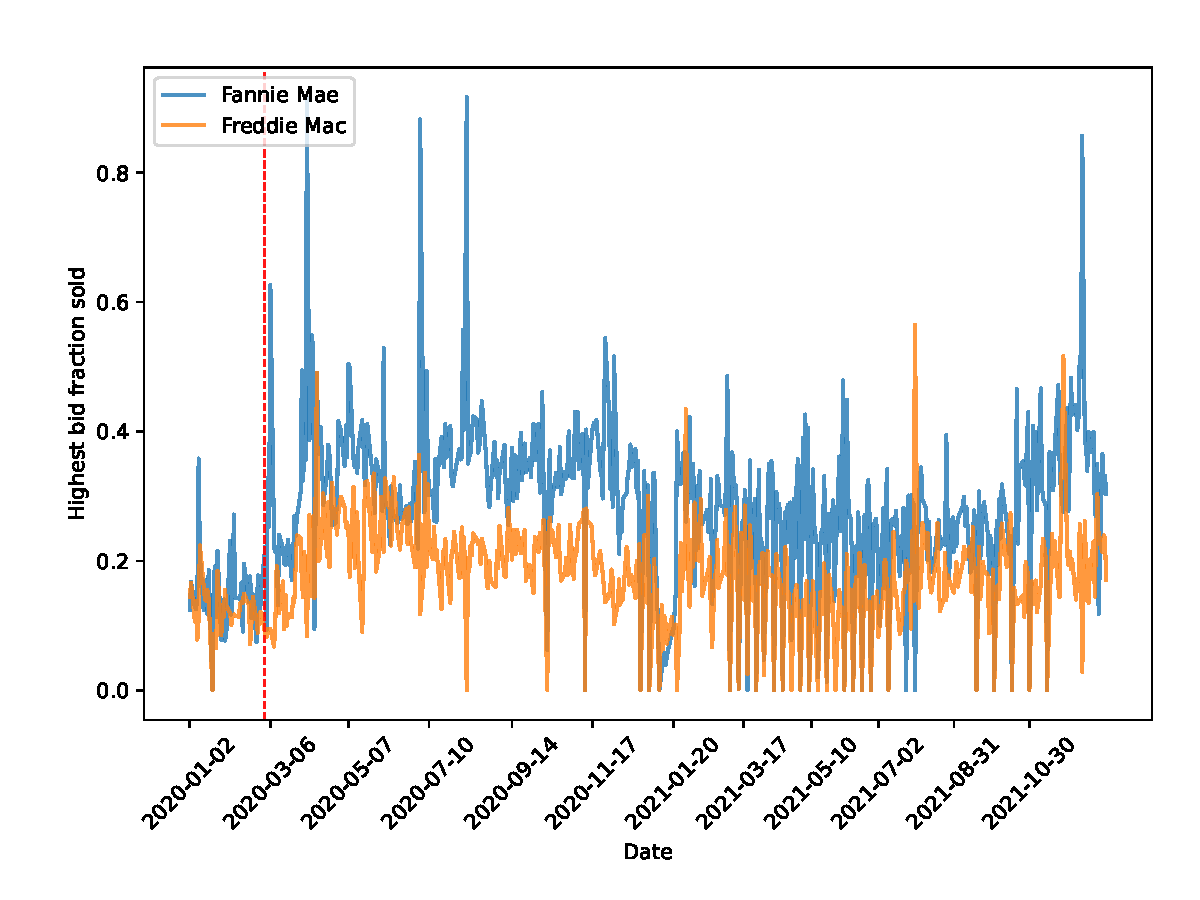
\includegraphics[width=0.998\textwidth]{../results/figures/sold_FreddieBid_mean_mat30_loan1_timeseries_nr_1_7.pdf}
      \caption{ Fraction of loans sold to GSE}
     \end{subfigure}
     \caption{OB auction  GSE response. } 
   \begin{minipage}{\textwidth}
      \footnotesize{\textit{Notes:} The figure shows time series of auction outcomes for Conforming loans with a 30-year maturity. The vertical lines is March 1.  } 
      \end{minipage}
\end{figure}


\pagebreak
\subsubsection{Comparison of note rates}

\begin{figure}[h]
  \centering
  \begin{subfigure}[b]{0.49\textwidth}
      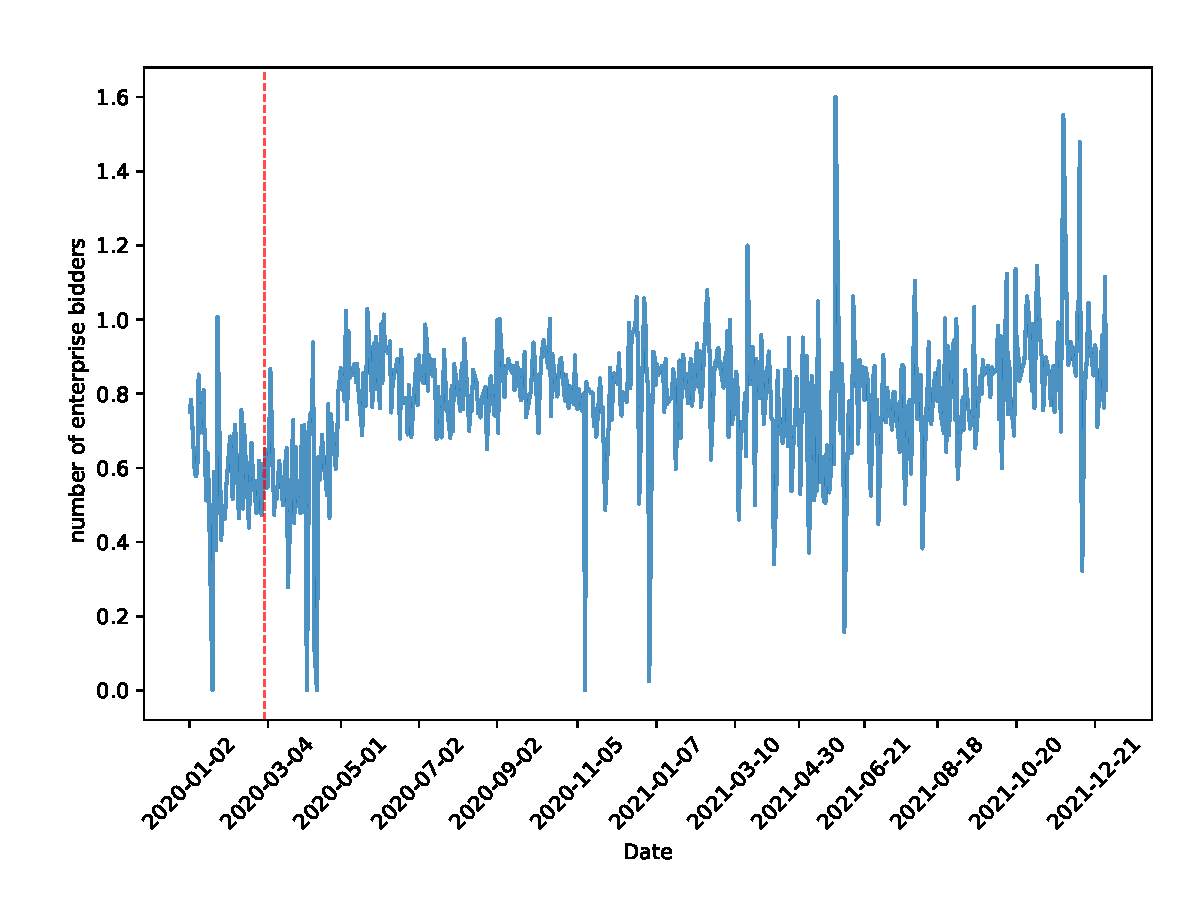
\includegraphics[width=0.998\textwidth]{../results/figures/Number of Enterprise Bidders_mean_mat30_loan1_timeseries_nr_3_3.75.pdf}
      \caption{Number of Enterprise Bids}
     \end{subfigure}
     \begin{subfigure}[b]{0.49\textwidth}
      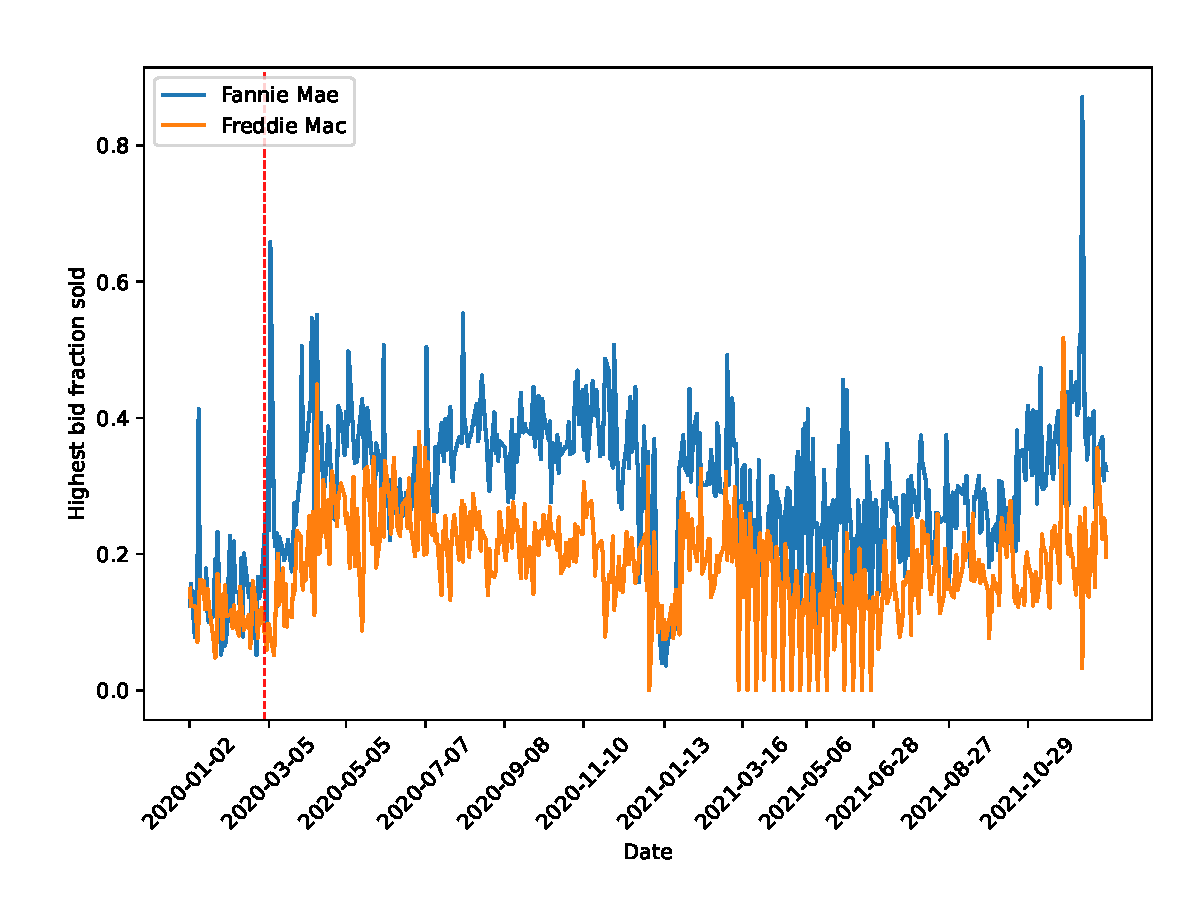
\includegraphics[width=0.998\textwidth]{../results/figures/sold_FreddieBid_mean_mat30_loan1_timeseries_nr_3_3.75.pdf}
      \caption{ Fraction of loans sold to GSE}
     \end{subfigure}
     \caption{OB auction  GSE response for note rates between 3\% and 3.75\%. } 
   \begin{minipage}{\textwidth}
      \footnotesize{\textit{Notes:} The figure shows time series of auction outcomes for Conforming loans with a 30-year maturity. The vertical lines is March 1.  } 
      \end{minipage}
\end{figure}

\begin{figure}[h]
  \centering
  \begin{subfigure}[b]{0.49\textwidth}
      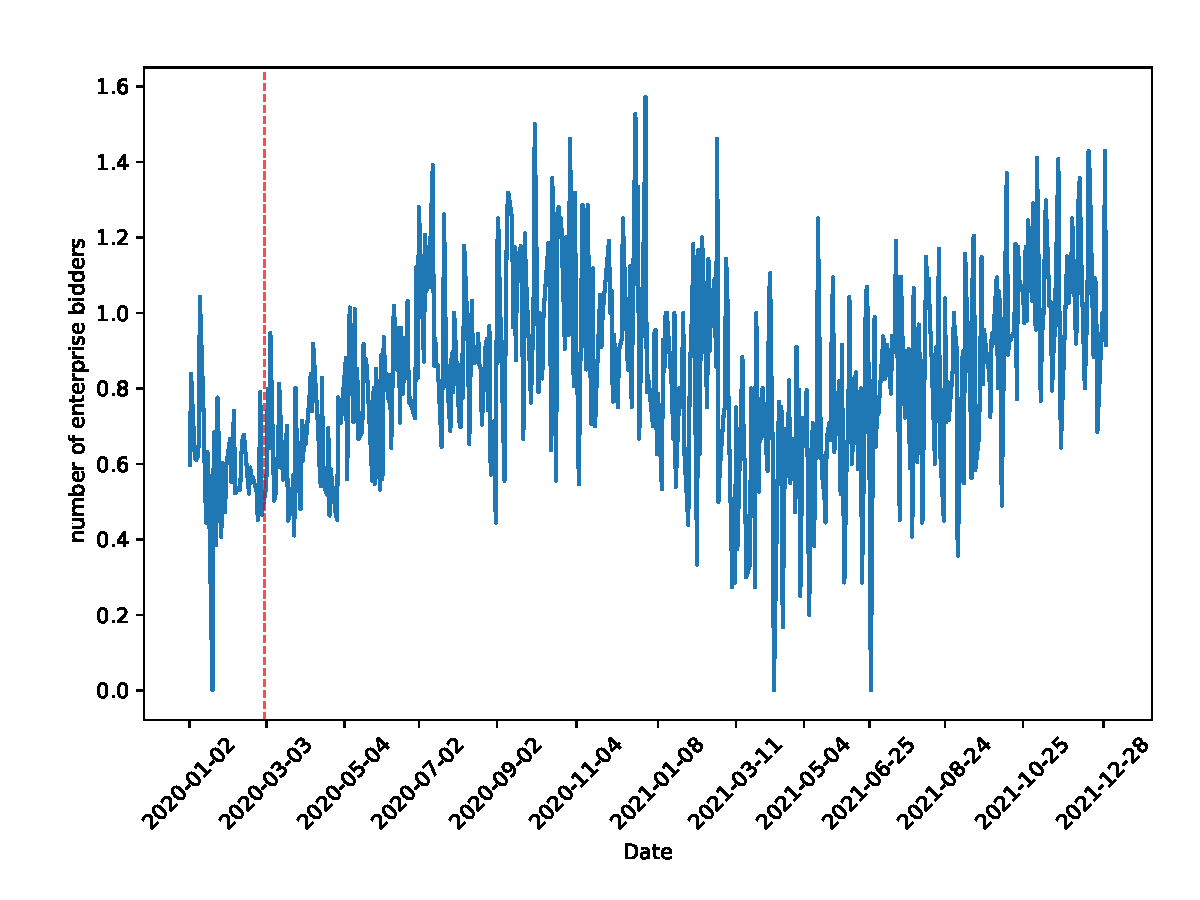
\includegraphics[width=0.998\textwidth]{../results/figures/Number of Enterprise Bidders_mean_mat30_loan1_timeseries_nr_4_4.75.pdf}
      \caption{Number of Enterprise Bids}
     \end{subfigure}
     \begin{subfigure}[b]{0.49\textwidth}
      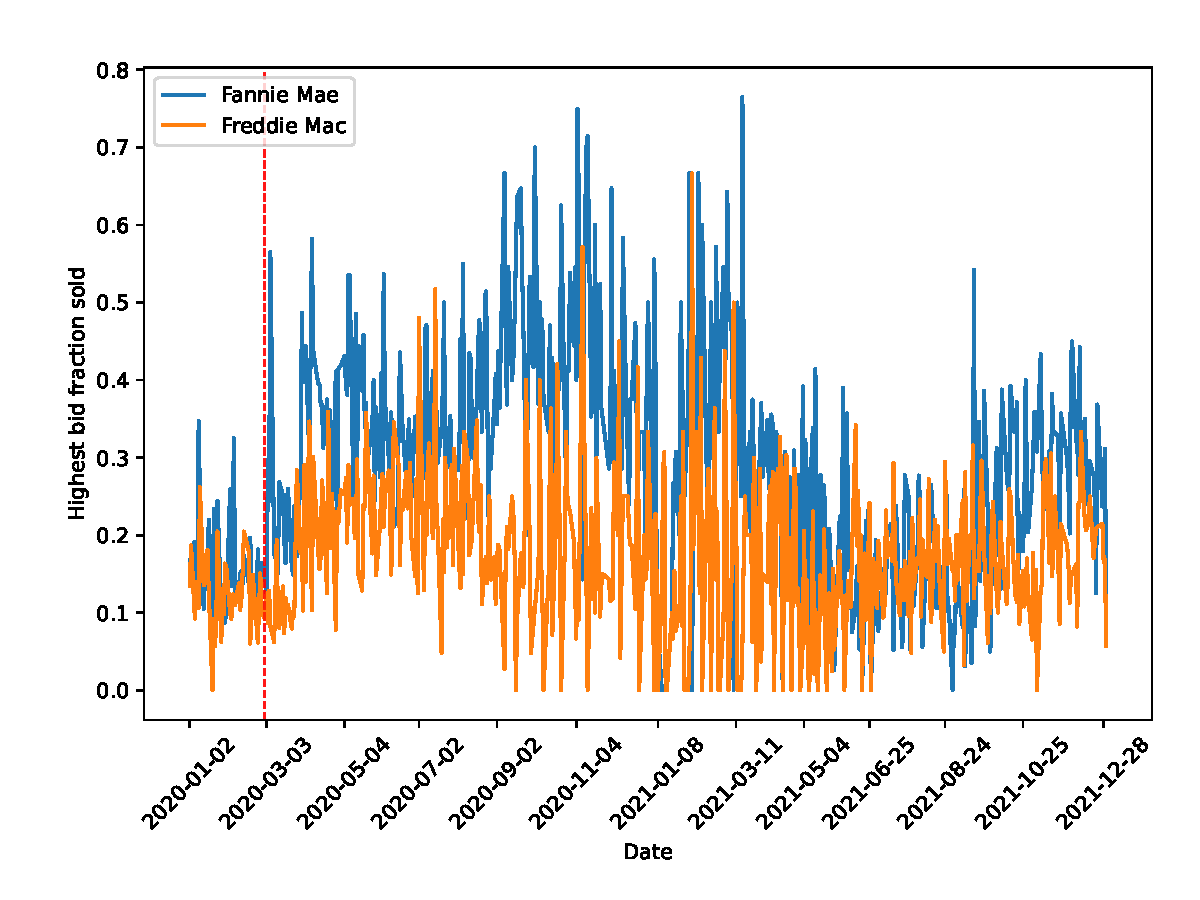
\includegraphics[width=0.998\textwidth]{../results/figures/sold_FreddieBid_mean_mat30_loan1_timeseries_nr_4_4.75.pdf}
      \caption{ Fraction of loans sold to GSE}
     \end{subfigure}
     \caption{OB auction  GSE response for note rates between 4\% and 4.75\%. }  
   \begin{minipage}{\textwidth}
      \footnotesize{\textit{Notes:} The figure shows the time series of auction outcomes for Conforming loans with a 30-year maturity. The vertical lines is March 1.  } 
      \end{minipage}
\end{figure}





\end{document}
